\documentclass[aps,prd,twocolumn,superscriptaddress,nofootinbib,longbibliography,floatfix,amsmath,amssymb,10pt]{revtex4-2}

\usepackage{mathptmx}
\usepackage{amsthm}
\usepackage{graphicx}
\usepackage{booktabs}
\usepackage{array}
\usepackage{xcolor}
\usepackage{enumitem}
\usepackage[colorlinks=true,linkcolor=blue!50!black,citecolor=blue!50!black,urlcolor=blue!50!black,bookmarksnumbered=true]{hyperref}
\usepackage{orcidlink}
\usepackage{microtype}
\usepackage{xurl}

\makeatletter
\AtBeginDocument{\def\NAT@bibsetup{\setlength{\labelwidth}{\z@}%
 \setlength{\labelsep}{0.5em}\setlength{\itemindent}{\z@}%
 \setlength{\listparindent}{\z@}\setlength{\topsep}{\z@}%
 \setlength{\parsep}{\z@}\NATx@bibsetup}}
\let\write@bibliographystyle\relax
\let\bibliography@latex\@gobble
\makeatother

\tolerance=2000
\emergencystretch=2em
\hbadness=2000
\hfuzz=1pt

\newtheorem{theorem}{Theorem}
\newtheorem{lemma}[theorem]{Lemma}
\newtheorem{proposition}[theorem]{Proposition}
\newtheorem{corollary}[theorem]{Corollary}
\newtheorem{conjecture}[theorem]{Conjecture}
\newtheorem*{theoremA}{Theorem A}
\newtheorem*{theoremB}{Theorem B}
\newtheorem*{theoremC}{Theorem C}
\newtheorem*{theoremD}{Theorem D}
\newtheorem*{theoremE}{Theorem E}
\newtheorem*{theoremF}{Theorem F}
\newtheorem*{theoremG}{Theorem G}
\theoremstyle{definition}
\newtheorem{definition}[theorem]{Definition}
\newtheorem{problem}[theorem]{Problem}
\theoremstyle{remark}
\newtheorem{remark}[theorem]{Remark}

\newcommand{\R}{\mathbb{R}}
\newcommand{\Z}{\mathbb{Z}}
\newcommand{\C}{\mathbb{C}}
\newcommand{\E}{\mathbb{E}}
\newcommand{\SU}{\mathrm{SU}}
\newcommand{\SO}{\mathrm{SO}}
\newcommand{\U}{\mathrm{U}}
\newcommand{\g}{\mathfrak{g}}
\newcommand{\Tr}{\operatorname{Tr}}
\newcommand{\ReTr}{\operatorname{Re}\operatorname{Tr}}
\newcommand{\Hess}{\operatorname{Hess}}
\newcommand{\Ric}{\operatorname{Ric}}
\newcommand{\Cov}{\operatorname{Cov}}
\newcommand{\Var}{\operatorname{Var}}
\newcommand{\dist}{\operatorname{dist}}
\newcommand{\diam}{\operatorname{diam}}
\newcommand{\ip}[2]{\langle #1,#2\rangle}

\setlength{\emergencystretch}{3em}
\begin{document}

\title{Sharp Curvature, Uniqueness and Finite-Box Criteria for Lattice
Yang--Mills Theory}

\author{Deep Bhattacharjee\,\orcidlink{0000-0003-0466-750X}}
\email{itsdeep@live.com}
\thanks{$*$\,Corresponding author. Second address:
\nolinkurl{d.bhattacharjee@erl-forschung.de}.}
\affiliation{Formerly, Electro-Gravitational Space Propulsion Laboratory
(EGSPL), Bhubaneswar, Odisha 751030, India}
\affiliation{Formerly, University of Calcutta, Senate House, 87/1 College
Street, Kolkata 700073, West Bengal, India}

\author{Ushashi Bhattacharya\,\orcidlink{0009-0002-2254-3914}}
\email{rai.bhattacharya.in@gmail.com}
\affiliation{Formerly, National Taiwan University, Taipei 106319, Taiwan}

\date{18 October 2026}

\begin{abstract}
\itshape
We prove unconditionally that the Hessian of the Wilson action on
$d$-dimensional lattice gauge fields is bounded by $4d$, and that $4d$ is
attained. Consequently lattice $\SU(N)$ Yang--Mills theory has a unique
infinite-volume state with a positive mass gap for $|\beta|<1/(8d)$, and
four-dimensional $\SU(2)$ theory has one for $\beta_W<1/(3\sqrt3)$. A
gauge-invariant finite-box criterion yields confinement. The continuum mass
gap remains open.
\par\medskip\upshape\noindent
\textit{2020 Mathematics Subject Classification.} Primary 81T25 (Quantum
field theory on lattices), 81T13 (Yang--Mills and other gauge theories in
quantum field theory); Secondary 82B20 (Lattice systems and systems on
graphs arising in equilibrium statistical mechanics), 60K35 (Interacting
random processes; statistical mechanics type models), 58J65 (Diffusion
processes and stochastic analysis on manifolds), 53C21 (Methods of global
Riemannian geometry; curvature restrictions), 47D07 (Markov semigroups and
applications to diffusion processes), 49Q22 (Optimal transportation), 22E30
(Analysis on real and complex Lie groups), 60J60 (Diffusion processes).
\end{abstract}

\keywords{lattice gauge theory; Bakry--\'Emery curvature; Dobrushin
uniqueness; mass gap}

\maketitle

\makeatletter
\renewcommand\l@subsection[2]{}
\renewcommand\l@subsubsection[2]{}
\makeatother
\tableofcontents

\section{Introduction}\label{sec:intro}

Wilson's lattice gauge theory~\cite{Wil74}\footnote{Wilson introduced the
lattice action to explain confinement: at strong coupling the expectation of
a large Wilson loop decays like the exponential of its area, which is the
statement that a static quark and antiquark are bound by a linear potential.
The Hamiltonian version, with continuous time and a lattice in space, is due
to Kogut and Susskind~\cite{KS75}; there the electric energy is the Laplacian
on each link group and the magnetic energy is the plaquette term, and the
mass gap is the gap above the ground state of this Hamiltonian. The two
formulations are related by the transfer matrix of Sec.~\ref{sec:transfer}.
Standard accounts of the lattice theory, its symmetries, its strong-coupling
expansion and its numerical simulation are the books of Montvay and
M\"unster~\cite{MM94} and of Gattringer and Lang~\cite{GL10}.} is where every attempt to
construct four-dimensional Yang--Mills theory begins. Its configurations are
assignments of a group element $Q_e$ of a compact group $G$ to each link $e$
of a lattice, its weight is $\exp(N\beta\sum_p\ReTr Q_p)$, a sum over
elementary squares (plaquettes), and the inverse coupling $\beta$ is the only
parameter.\footnote{Throughout, $Q_p$ is the ordered product of the four link
variables around the plaquette $p$, so that $\ReTr Q_p=N$ exactly when the
field is flat on $p$. Large $\beta$ favours flat fields; this is the weak
coupling regime, which is the one relevant for the continuum limit.} When
$\beta$ is small the theory is understood: the cluster expansion of
Osterwalder and Seiler~\cite{OSei78,Sei82} produces a positive gap in the
spectrum of the transfer matrix and exponential decay of correlations.
Shen, Zhu and Zhu~\cite{SZZ23} found a second route, through the geometry of
the configuration space: they verified the Bakry--\'Emery
criterion~\cite{BE85,BGL14} on the product manifold $G^E$ and obtained
log-Sobolev inequalities uniform in the volume, uniqueness of the
infinite-volume limit and decay of correlations. The strength of that route
is set by one number, the constant in the bound
\begin{equation}\label{eq:szzbound}
|\Hess S_0(v,v)|\le 8(d-1)\,|v|^2
\end{equation}
for the Hessian of the Wilson action $S_0=\sum_p\ReTr Q_p$ in $d$ dimensions.
The same constant reappears in later work on Langevin dynamics, on the area
law and on the Yang--Mills--Higgs model~\cite{CNS25b,Nis25,SSZ26}.

This paper has three aims. The first is to find the best constant
in~\eqref{eq:szzbound}. The second is to carry that constant, and a sharper
analysis of the single-link law of $\SU(2)$, through to uniqueness and to a
positive lattice mass gap. The third is structural: a criterion, checkable
in one finite box, that produces decay at all scales for gauge fields, and an
honest account of what still separates all of this from the continuum mass
gap.

\subsection{The Hessian}

The bound~\eqref{eq:szzbound} is obtained plaquette by plaquette. The cross
terms between the four links of one plaquette, however, are not independent
across the lattice: summed over all plaquettes they reassemble into the
square of a covariant divergence, which has a sign. Keeping that square
gives the sharp constant.

\begin{theoremA}[Sharp Hessian bound]
Let $d\ge2$, and let $G$ be one of the groups $\SU(N)$, $\SO(N)$ or $\U(N)$.
For every gauge field $Q$ on $\Z^d$ or on a torus and every square-summable
tangent vector $v=(X_eQ_e)_e$,
\[
\pm\Hess S_0(v,v)+\sum_x|D_xX|^2\le 4d\,|v|^2,
\]
where $D_xX$ is the covariant divergence~\eqref{eq:divergence}. In
particular $|\Hess S_0(v,v)|\le 4d\,|v|^2$, and for every $N\ge2$ and $d\ge2$
the constant $4d$ is attained with both signs.
\end{theoremA}

For $d=2$ the two constants coincide; for $d=3$ and $d=4$ they are $12$
against $16$ and $16$ against $24$.\footnote{We searched arXiv and the
journal literature up to October 2026 for the constant $4d$ and did not find
it. The bound $8(d-1)$ is stated in~\cite[Lemma~4.1]{SZZ23} and used
in~\cite{CNS25b,Nis25,SSZ26}.} The two extremal fields are drawn in
Fig.~\ref{fig:extremal}.

\subsection{Strong coupling}

The Ricci curvature of $\SU(N)$ in the metric of Sec.~\ref{sec:setting} is
$N/2$, and that of $\SO(N)$ is $(N-2)/4$. Subtracting the Hessian bound gives
the Bakry--\'Emery constant directly.

\begin{theoremB}[Curvature regime]
Let $G=\SU(N)$ and $|\beta|<1/(8d)$, or $G=\SO(N)$ with $N\ge3$ and
$|\beta|<(N-2)/(16dN)$. The finite-volume Wilson measures satisfy the
Bakry--\'Emery condition with a constant $K>0$ that depends neither on the
volume, nor on the boundary condition, nor on the configuration. They
satisfy log-Sobolev and Poincar\'e inequalities uniform in the volume, and
every infinite-volume limit has exponentially decaying correlations of local
functions.
\end{theoremB}

\begin{theoremC}[The limit of the curvature method]
For $G=\SU(N)$ on every torus of even side,
\[
\inf_Q\lambda_{\min}\bigl(\Ric-N\beta\Hess S_0(Q)\bigr)=\tfrac N2-4dN|\beta|.
\]
No Bakry--\'Emery argument with a lower bound uniform over configurations,
in the bi-invariant metric, reaches beyond $|\beta|=1/(8d)$.
\end{theoremC}

The curvature bound also controls a coupling of two Langevin dynamics. Shen,
Zhu and Zhu built such a coupling and needed a second, separate estimate to
make it contract in a weighted metric; that estimate cost a factor of two in
the range of $\beta$. Applying Theorem~A to the whole weighted sum, rather
than link by link, removes the loss.

\begin{theoremD}[Uniqueness on the whole curvature range]
Under the hypotheses of Theorem~B the Langevin dynamics of the Wilson
measure on $\Z^d$ has exactly one invariant probability measure $\mu$. The
Wilson measures on the periodic tori $(\Z/L\Z)^d$ converge to $\mu$ as
$L\to\infty$, and every initial law converges to $\mu$ exponentially fast in a
weighted Wasserstein distance.
\end{theoremD}

\subsection{SU(2) beyond the curvature range}

For $\SU(2)$ the conditional law of one link given all the others is a von
Mises--Fisher law on the three-sphere, and its moments are explicit. A
Dobrushin argument in the chordal metric then goes past the curvature range.

\begin{theoremE}[Uniqueness for $\SU(2)$]
Let $G=\SU(2)$ and $|\beta|<1/(4\sqrt3\,(d-1))$. The Wilson theory on $\Z^d$
has exactly one infinite-volume Gibbs measure, and its truncated
correlations of local Lipschitz functions decay exponentially with every rate
$\lambda<-\log\bigl(4\sqrt3(d-1)|\beta|\bigr)$. At $d=4$ the range is
$\beta_W<1/(3\sqrt3)\approx0.1925$. No single-link Wasserstein--Dobrushin
argument, in the chordal or the geodesic metric, reaches beyond
$|\beta|=1/(6(d-1))$, that is $\beta_W=2/9$ at $d=4$.
\end{theoremE}

Here $\beta_W=N^2\beta$ is the Wilson coupling of the physics
literature.\footnote{We follow the normalisation of Shen, Zhu and Zhu~\cite{SZZ23}:
the weight is $\exp(N\beta\sum_p\ReTr Q_p)$. The physics literature writes
$\exp(\frac{\beta_W}N\sum_p\ReTr Q_p)$, so $\beta_W=N^2\beta$, and for
$\SU(2)$, $\beta_W=4\beta$.} Between $1/(3\sqrt3)$ and $2/9$ the remaining
question is a single inequality on the three-sphere,
Conjecture~\ref{conj:quarter}, which we prove in three of its four regimes.

\subsection{A lattice mass gap}

Reflection positivity turns decay of correlations in the time direction into
a gap in the spectrum of the transfer matrix.

\begin{theoremF}[Lattice mass gap]
In the range of Theorem~B, and for $\SU(2)$ in the range of Theorem~E, the
infinite-volume state is reflection positive and its transfer matrix
$\mathbb T$ has a spectral gap: the spectrum of $\mathbb T$ on the
orthogonal complement of the vacuum lies in $[0,e^{-m}]$ with $m>0$. For
$\SU(2)$ one may take $m=-\log\bigl(4\sqrt3(d-1)|\beta|\bigr)$, which at
$d=4$ reads $m=-\log(3\sqrt3\,\beta_W)$.
\end{theoremF}

This is a gap in lattice units at fixed lattice spacing. It is not the mass
gap of the continuum theory: our earlier paper~\cite{BB26} shows that no
inequality of this kind, uniform in the spacing and stated in lattice units,
can produce the continuum gap, because the physical gap in lattice units
must vanish like the spacing.

\subsection{A finite-box criterion}

For spin systems, Dobrushin and Shlosman showed that a single finite
computation implies uniqueness and decay at all scales~\cite{DS85}.\footnote{Dobrushin's
original criterion~\cite{Dob68,Dob70} compares the conditional laws at a
single site: if the total influence $\sum_y\kappa(x,y)$ of all other sites on
the conditional law at $x$ is below $1$, the Gibbs measure is unique and
correlations decay. It is local in space but global in the interaction
strength, and it fails before the critical point. Dobrushin and Shlosman
replaced the single site by a finite box and asked that the influence of the
boundary on the box, averaged over the box, be below its volume; this
condition holds in the whole high-temperature phase of many models and is
equivalent there to several other forms of complete analyticity. Expositions
of the single-site theory are in the books of Georgii~\cite{Geo11},
Simon~\cite{Sim93} and Friedli and Velenik~\cite{FV17}; the coupling
formulation used below is that of Ref.~\cite{Geo11}, Ch.~8.} Gauge
fields need three changes: boundary data are holonomies,
gauge-equivalent boundary conditions must be identified, and disagreement
is measured after an interior gauge alignment. With these changes:

\begin{theoremG}[Gauge-invariant finite-box criterion]
For every compact group $G$ and every finite-range gauge-invariant
interaction, the finite-box inequality of Definition~\ref{def:gds} implies
uniqueness of the infinite-volume Gibbs measure, exponential decay of all
truncated correlations, and the same decay on every large torus, uniformly
in its size and in every 't~Hooft twist sector. Its box-hereditary form
implies Wilson's area law.
\end{theoremG}

Two-dimensional $\SU(2)$ theory meets the criterion at every coupling
(Proposition~\ref{prop:2d}). Four-dimensional $\U(1)$ theory at weak coupling
cannot meet it, because that theory is massless~\cite{Gut80,FS82}; a
criterion that did not fail there would be wrong.

\subsection{What is proved and what is not}

Figure~\ref{fig:thresholds} places the thresholds on one axis, and
Table~\ref{tab:gaps} in Sec.~\ref{sec:open} lists the gaps between this paper
and the continuum mass gap, with the status of each. Everything stated as a
theorem, proposition or lemma is proved here, by hand, without conditions.
The mass gap of the continuum four-dimensional theory is not proved here, at
intermediate lattice coupling or in the continuum. What is missing is stated
precisely as Problem~\ref{prob:crossover}.

\begin{figure*}[t]
\centering
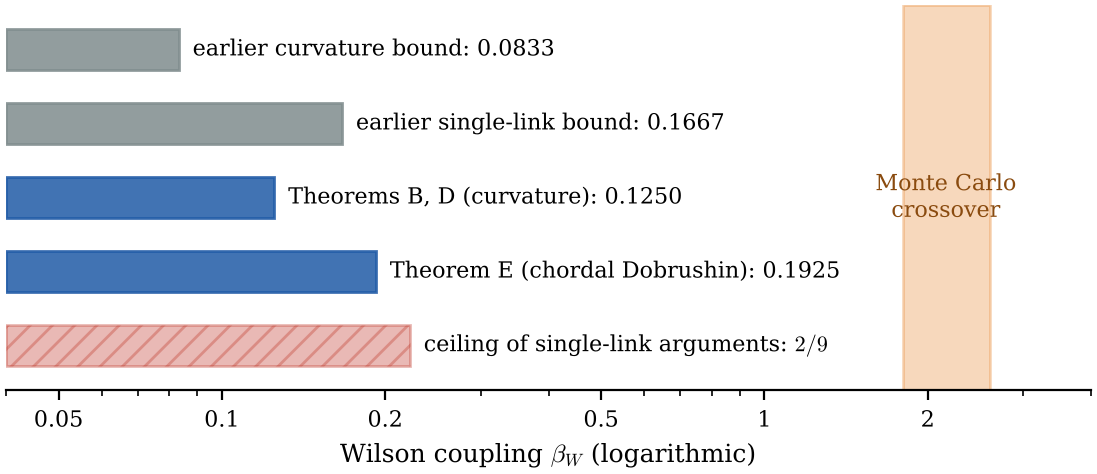
\includegraphics[width=0.96\textwidth]{figures/fig_thresholds.png}
\caption{Thresholds for four-dimensional $\SU(2)$ in the Wilson coupling
$\beta_W$, on a logarithmic scale. Grey marks: the earlier curvature bound
$1/12$ from~\eqref{eq:szzbound} and the authors' earlier single-link bound
$1/6$. Blue: Theorems~B, D (curvature, $1/8$) and Theorem~E (chordal
Dobrushin, $1/(3\sqrt3)$). Red: the ceiling $2/9$ of all single-link
Wasserstein--Dobrushin arguments, reached if Conjecture~\ref{conj:quarter}
holds. Orange: the region where Monte Carlo simulations place the crossover to
weak coupling, which plays no role in any proof.}
\label{fig:thresholds}
\end{figure*}

\section{Setting}\label{sec:setting}

Let $G\in\{\SU(N),\SO(N),\U(N)\}$ with Lie algebra $\g$. We use the inner
product $\ip XY=-\Tr(XY)=\ReTr(X^*Y)$ on $\g$ and the bi-invariant metric it
induces on $G$. In this metric
\begin{equation}\label{eq:ricci}
\Ric_{\SU(N)}=\tfrac N2,\qquad \Ric_{\SO(N)}=\tfrac{N-2}4.
\end{equation}
Indeed $\Ric(X,X)=-\frac14B(X,X)$ for the Killing form $B$ of a compact group
with a bi-invariant metric~\cite{Mil76},\footnote{For a bi-invariant metric
the Levi-Civita connection on left-invariant fields is $\nabla_XY=\frac12[X,Y]$,
so $R(X,Y)Z=-\frac14[[X,Y],Z]$ and the sectional curvature of the plane
spanned by orthonormal $X,Y$ is $\frac14|[X,Y]|^2\ge0$. Summing over an
orthonormal basis $(Y_j)$ gives $\Ric(X,X)=\frac14\sum_j|[X,Y_j]|^2=
-\frac14\Tr(\mathrm{ad}_X^2)=-\frac14B(X,X)$; this is the bi-invariant case of
Milnor's formulas for left-invariant metrics~\cite{Mil76}. On
$\mathfrak{su}(N)$ one has $\Tr(\mathrm{ad}_X^2)=2N\Tr X^2$, because
$\mathrm{ad}_X$ extends to $\mathfrak{gl}(N,\C)=\mathfrak{sl}(N,\C)\oplus\C1$,
where it vanishes on the centre and acts as $X\otimes1-1\otimes X^T$, whose
square has trace $2N\Tr X^2-2(\Tr X)^2$; for traceless $X$ this is $2N\Tr X^2$. Since
$-\Tr X^2=|X|^2$ in our normalisation, $\Ric=N/2$. The same computation on
antisymmetric matrices gives $(N-2)\Tr X^2$ and $\Ric=(N-2)/4$.} and $B(X,X)=2N\Tr X^2$ on $\mathfrak{su}(N)$,
$B(X,X)=(N-2)\Tr X^2$ on $\mathfrak{so}(N)$.\footnote{For $\U(N)$ the centre
contributes a flat direction, so $\Ric_{\U(N)}$ is not bounded below by a
positive constant, and Theorem~B is not stated for $\U(N)$. Theorem~A holds
for $\U(N)$ as stated.} With this metric $\SU(2)$ is the round three-sphere
of radius $\sqrt2$.

Let $\Lambda\subset\Z^d$ be a finite box or a torus, $E$ its set of
positively oriented links and $P$ its set of plaquettes. The plaquette $p$
with base point $x$ in the plane of the directions $\mu<\nu$ has the links
\[
e_1=(x,\mu),\quad e_2=(x+\hat\mu,\nu),\quad e_3=(x+\hat\nu,\mu),\quad
e_4=(x,\nu),
\]
and $Q_p=Q_{e_1}Q_{e_2}Q_{e_3}^*Q_{e_4}^*$. The Wilson measure is
\begin{equation}\label{eq:wilson}
\begin{gathered}
d\mu_{\Lambda,\beta}(Q)=Z^{-1}e^{S(Q)}\prod_e dQ_e,\\
S=N\beta S_0,\qquad S_0=\sum_{p\in P}\ReTr Q_p,
\end{gathered}
\end{equation}
with normalised Haar measure $dQ_e$; on a box the links outside $\Lambda$ are
frozen to a boundary condition.

A tangent vector at $Q$ is $v=(X_eQ_e)_e$ with $X_e\in\g$, and
$|v|^2=\sum_e|X_e|^2$. Since $t\mapsto e^{tX}Q$ is a geodesic of the
bi-invariant metric, $\Hess S_0(v,v)=\frac{d^2}{dt^2}S_0\bigl((e^{tX_e}Q_e)_e
\bigr)|_{t=0}$.\footnote{On a compact Lie group with a bi-invariant metric
the one-parameter subgroups and their translates are exactly the geodesics.
The Hessian of a function $f$ at $Q$ in the direction $v$ is therefore the
second derivative of $f$ along the geodesic through $Q$ with velocity $v$,
and the polarisation identity recovers the bilinear form.} On $\Z^d$ the
Hessian at any field is a bounded quadratic form on square-summable vectors,
because it is a sum of finite-range blocks of uniformly bounded size.

\section{The sharp Hessian bound}\label{sec:hessian}

\subsection{One plaquette}

Fix a plaquette $p$ and a tangent vector $v=(X_eQ_e)$. Transport the four
link vectors to the base point of $p$:
\begin{equation}\label{eq:transport}
Y_1=X_{e_1},\ \ Y_2=Q_{e_1}X_{e_2}Q_{e_1}^*,\ \
Y_3=Q_{e_4}X_{e_3}Q_{e_4}^*,\ \ Y_4=X_{e_4},
\end{equation}
and write $W=Q_p$. Then the perturbed plaquette variable is
$Q_p(t)=e^{tY_1}e^{tY_2}We^{-tY_3}e^{-tY_4}$ (Appendix~\ref{app:hessian}), and
\begin{equation}\label{eq:fp}
\begin{split}
f_p:={}&\frac{d^2}{dt^2}\ReTr Q_p(t)\Big|_{t=0}\\
={}&\sum_{i=1}^4\ReTr(Y_i^2W)+2\ReTr(Y_1Y_2W)+2\ReTr(Y_3Y_4W)\\
&-2\sum_{i\in\{1,2\},\,j\in\{3,4\}}\ReTr(Y_iWY_j),
\end{split}
\end{equation}
so that $\Hess S_0(v,v)=\sum_pf_p$.

\subsection{The covariant divergence}

The covariant divergence of $X$ at a vertex $x$ is
\begin{equation}\label{eq:divergence}
D_xX=\sum_{\mu=1}^d\Bigl[X_{x,\mu}-Q_{x-\hat\mu,\mu}^*X_{x-\hat\mu,\mu}
Q_{x-\hat\mu,\mu}\Bigr]\in\g .
\end{equation}
Each summand is the vector of a link with an end at $x$, transported to $x$,
with sign $+$ for an outgoing and $-$ for an incoming link.\footnote{At the
identity field, $D_xX$ is the lattice divergence of the Lie-algebra valued
one-form $X$, and $\sum_x|D_xX|^2$ is the gauge-fixing term of the Lorenz
gauge. The point of Theorem~A is that this positive term is hidden inside the
Hessian of the Wilson action at every field, not only near the identity.} The
corner form of $p$ is
\begin{equation}\label{eq:corner}
c_p=2\ip{Y_1}{Y_4}-2\ip{Y_1}{Y_2}+2\ip{Y_2}{WY_3W^*}-2\ip{Y_3}{Y_4}.
\end{equation}

\begin{lemma}\label{lem:divergence}
For every field $Q$ and every square-summable $X$,
\[
\sum_x|D_xX|^2=2|X|^2+\sum_pc_p+\sum_{x,\mu}\kappa_{x,\mu},
\]
where
\[
\kappa_{x,\mu}=-2\bigl\langle X_{x,\mu},Q^*_{x-\hat\mu,\mu}X_{x-\hat\mu,\mu}
Q_{x-\hat\mu,\mu}\bigr\rangle,
\]
and $\sum_{x,\mu}|\kappa_{x,\mu}|\le 2|X|^2$.
\end{lemma}

\begin{proof}
The vector $D_xX$ is a signed sum of $2d$ vectors, one for each end of a link
at $x$. Expanding $|D_xX|^2$ and summing over $x$ gives three kinds of term.
The squares contribute $2|X|^2$, since every link has two ends. The cross
term between the outgoing and the incoming link in the same direction $\mu$
is $\kappa_{x,\mu}$. The cross terms between ends in two perpendicular
directions $\mu\ne\nu$ are in bijection with pairs consisting of a plaquette
of the plane $\mu\nu$ and one of its corners at $x$: through $x$ pass four
plaquettes of that plane, one for each choice of two signs. Appendix~\ref{app:hessian}
identifies the four corner terms of each plaquette with the four terms
of~\eqref{eq:corner}. Finally
$|\kappa_{x,\mu}|\le|X_{x,\mu}|^2+|X_{x-\hat\mu,\mu}|^2$ by the
Cauchy--Schwarz inequality, and the sum over $(x,\mu)$ counts every link
twice.
\end{proof}

\begin{figure*}[t]
\centering
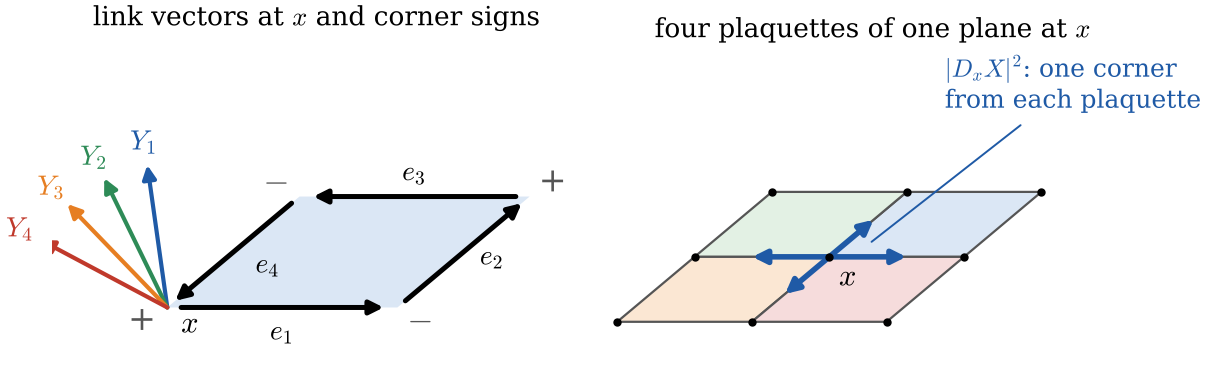
\includegraphics[width=0.96\textwidth]{figures/fig_plaquette.png}
\caption{Left: a plaquette with its links $e_1,\dots,e_4$, the link vectors
$Y_1,\dots,Y_4$ transported to the base point $x$, and the sign with which
each corner enters the corner form~\eqref{eq:corner}. Right: the four
plaquettes of one plane through a vertex $x$; each contributes one corner to
$|D_xX|^2$, which is how the cross terms of the Hessian reassemble into the
divergence.}
\label{fig:plaquette}
\end{figure*}

\subsection{A local inequality}

\begin{lemma}\label{lem:local}
For every $N$, every $W\in\U(N)$ and all $Y_1,\dots,Y_4\in\mathfrak u(N)$,
\[
\pm f_p+c_p\le 2\sum_{i=1}^4|Y_i|^2 .
\]
\end{lemma}

\begin{proof}
Replacing $W$ by $-W$ changes the sign of $f_p$ and leaves $c_p$ unchanged,
so it suffices to prove the inequality with the sign $+$. Write $W=VDV^*$
with $V$ unitary and $D=\operatorname{diag}(w_1,\dots,w_N)$, $|w_a|=1$.
Replacing every $Y_i$ by $V^*Y_iV$ changes neither side, so we may assume
$W=D$. Every term of $f_p$ and of $c_p$ is then a sum over positions $(a,b)$
of products of the entries $(Y_i)_{ab}$, $(Y_j)_{ba}$ or
$\overline{(Y_i)_{ab}}$, $(Y_j)_{ab}$, with phases from $D$. Since
$(Y_i)_{ba}=-\overline{(Y_i)_{ab}}$, each term couples only the positions
$(a,b)$ and $(b,a)$. Hence the form $F=2\sum|Y_i|^2-f_p-c_p$ is an orthogonal
sum of blocks: one for each diagonal position $a$, in the variables
$(Y_i)_{aa}=\mathrm iy_i$ with $y\in\R^4$, and one for each unordered pair
$a\ne b$, in the variables $z_i=(Y_i)_{ab}\in\C$. Appendix~\ref{app:hessian}
computes these blocks:
\[
F_{aa}=(y_1+y_3)^2+(y_2+y_4)^2+(1+\cos\varphi)(y_1+y_2-y_3-y_4)^2
\]
with $w_a=e^{\mathrm i\varphi}$, and $F_{ab}=z^*M(m,\theta)z$ with
$w_{a,b}=e^{\mathrm i(\chi\pm\theta)}$, $m=\cos\chi$, and a Hermitian matrix
$M$ affine in $m$ that satisfies $M(-1,\theta)=M(1,\theta+\pi)$. Therefore
$M(m,\theta)=\frac{1+m}2M(1,\theta)+\frac{1-m}2M(1,\theta+\pi)$, and after a
diagonal unitary change of variables $z=\Delta u$ and with $c=\cos(\theta/2)$,
\begin{multline*}
z^*M(1,\theta)z=2c^2\bigl(|u_1+u_3|^2+|u_2+u_4|^2\bigr)\\
+(1+c)^2|u_1+u_2-u_3-u_4|^2+(1-c)^2|u_1-u_2-u_3+u_4|^2 .
\end{multline*}
Every block is a sum of squares, so $F\ge0$.
\end{proof}

The pairing of $(a,b)$ with $(b,a)$ is essential.\footnote{The blocks of the
ordered positions $(a,b)$ and $(b,a)$, taken separately, are not positive
semidefinite: at $w_a=-1$, $w_b=1$ each of them has a negative eigenvalue.
Only after the identification $(Y)_{ba}=-\overline{(Y)_{ab}}$, which uses
that the $Y_i$ are anti-Hermitian, does the form become a sum of squares.}

\subsection{Proof of Theorem A}

\begin{proof}[Proof of the upper bound]
By density it suffices to take $X$ finitely supported. Every link lies in
$2(d-1)$ plaquettes and $|Y_i|=|X_{e_i}|$, so summing Lemma~\ref{lem:local}
over $p$ gives $\sum_p(\pm f_p+c_p)\le4(d-1)|X|^2$. By
Lemma~\ref{lem:divergence},
$\sum_pc_p=\sum_x|D_xX|^2-2|X|^2-\sum\kappa\ge\sum_x|D_xX|^2-4|X|^2$. Hence
\[
\pm\Hess S_0(v,v)\le4(d-1)|X|^2+4|X|^2-\sum_x|D_xX|^2. \qedhere
\]
\end{proof}

\begin{proof}[Proof of sharpness]
Let the torus have even side and let $X_{x,\mu}=(-1)^{|x|}\varepsilon_\mu T$
with $|x|=\sum_\nu x_\nu$, a vector $\varepsilon\in\R^d$ with
$\sum_\mu\varepsilon_\mu=0$, and $0\ne T\in\g$.

\emph{The sign $-$.} At the identity field $W=1$ and $Y_i=X_{e_i}$,
and~\eqref{eq:fp} becomes $f_p=\Tr\bigl((Y_1+Y_2-Y_3-Y_4)^2\bigr)
=-|Y_1+Y_2-Y_3-Y_4|^2$. For the plaquette at $x$ in the plane $\mu\nu$,
$Y_1+Y_2-Y_3-Y_4=2(-1)^{|x|}(\varepsilon_\mu-\varepsilon_\nu)T$. Each vertex
therefore contributes
\[
\begin{aligned}
-4|T|^2\sum_{\mu<\nu}(\varepsilon_\mu-\varepsilon_\nu)^2
&=-4|T|^2\Bigl(d|\varepsilon|^2-\bigl(\textstyle\sum_\mu\varepsilon_\mu
\bigr)^2\Bigr)\\
&=-4d|\varepsilon|^2|T|^2,
\end{aligned}
\]
while it carries $|\varepsilon|^2|T|^2$ of $|X|^2$. So
$\Hess S_0(v,v)=-4d|X|^2$. Moreover $D_xX=2(-1)^{|x|}(\sum_\mu
\varepsilon_\mu)T=0$, so the inequality of Theorem~A is an equality.

\emph{The sign $+$.} Let $z=\operatorname{diag}(-1,-1,1,\dots,1)$, which lies
in $\SU(N)$, $\SO(N)$ and $\U(N)$, and $Q_{x,\mu}=z^{\sum_{\lambda<\mu}
x_\lambda}$, which is well defined on an even torus since $z^2=1$. For the
plaquette at $x$ in the plane $\mu<\nu$ one finds $Q_{e_1}=Q_{e_3}=
z^{\sum_{\lambda<\mu}x_\lambda}$, $Q_{e_4}=z^{\sum_{\lambda<\nu}x_\lambda}$ and
$Q_{e_2}=zQ_{e_4}$, so every plaquette variable equals $z$. Take the same $X$
with $T$ supported in the upper left $2\times2$ block, so that $T$ commutes
with $z$ and $zT=-T$. All transports act trivially on $T$, every term
of~\eqref{eq:fp} changes sign relative to the identity field, and so
$\Hess S_0(v,v)=+4d|X|^2$ and again $D_xX=0$.
\end{proof}

\begin{figure*}[t]
\centering
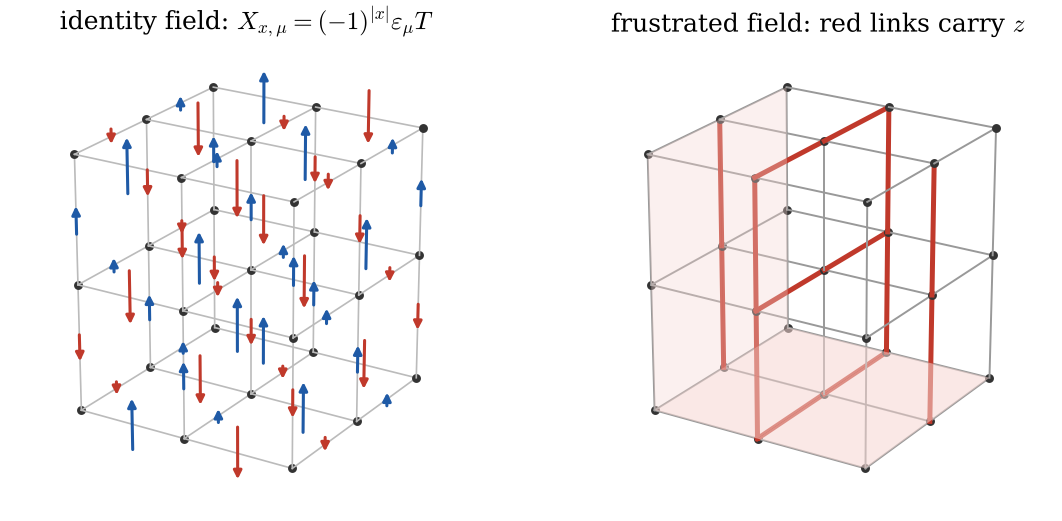
\includegraphics[width=0.96\textwidth]{figures/fig_extremal.png}
\caption{The two fields at which $\pm\Hess S_0=4d$. Left: the identity field
with the checkerboard tangent vector $X_{x,\mu}=(-1)^{|x|}\varepsilon_\mu T$,
$\sum_\mu\varepsilon_\mu=0$, drawn on a $3\times3\times3$ block (arrows of
alternating orientation, lengths proportional to $\varepsilon_\mu$). Right:
the frustrated field $Q_{x,\mu}=z^{\sum_{\lambda<\mu}x_\lambda}$ with
$z=\operatorname{diag}(-1,-1,1,\dots)$; red links carry $z$, and every
plaquette has holonomy $z$ (two faces of the block are shaded).}
\label{fig:extremal}
\end{figure*}

Figure~\ref{fig:spectrum} compares the bound with the spectrum of the
Hessian computed numerically for $\SU(2)$ on the torus $(\Z/4\Z)^3$. At
random fields the spectrum fills a part of $[-12,12]$; at the two extremal
fields it reaches the end points.

\begin{figure*}[t]
\centering
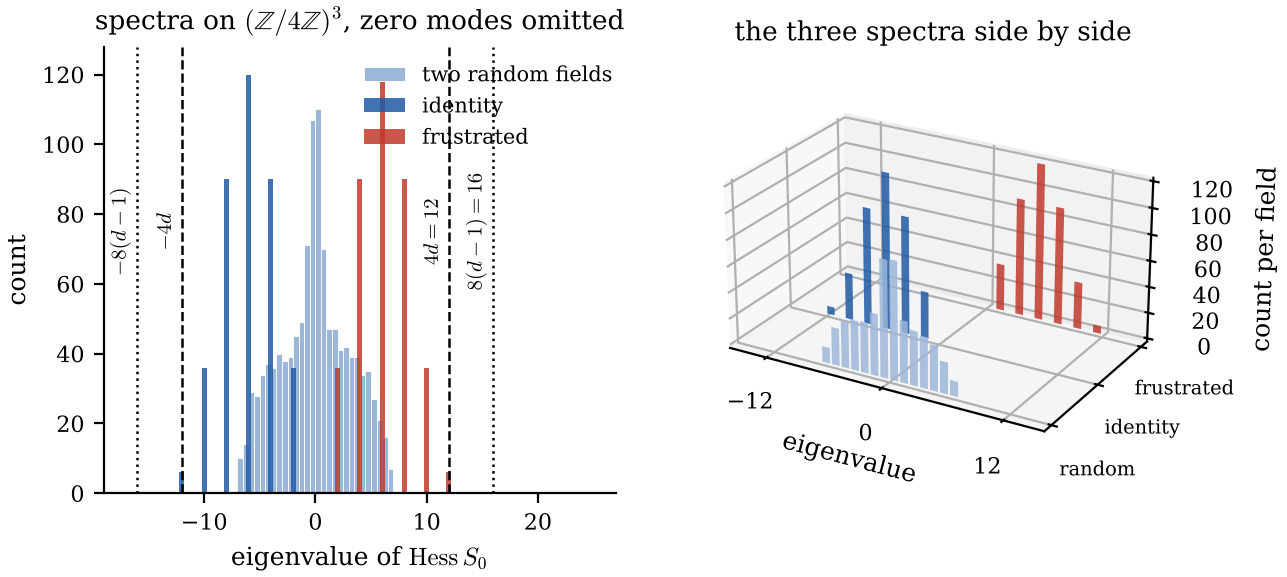
\includegraphics[width=0.96\textwidth]{figures/fig_spectrum.png}
\caption{Eigenvalues of $\Hess S_0$ for $\SU(2)$ on $(\Z/4\Z)^3$
($d=3$, $576$ eigenvalues per field). Histogram: two random Haar fields.
Solid bars: the identity field (left) and the frustrated field (right). The
dashed lines are Theorem~A ($\pm4d=\pm12$); the dotted lines are the earlier
bound~\eqref{eq:szzbound} ($\pm8(d-1)=\pm16$). The identity and frustrated
spectra touch $-12$ and $+12$. Right: the same three spectra in depth, the
random histogram divided by two so that every row counts one field; the
spectrum of the frustrated field is the reflection of that of the identity
field on this torus.}
\label{fig:spectrum}
\end{figure*}

\section{Consequences of the curvature bound}\label{sec:be}

\begin{proof}[Proof of Theorem B]
By Theorem~A,
\[
|\Hess S(v,v)|=N|\beta|\,|\Hess S_0(v,v)|\le4dN|\beta|\,|v|^2 .
\]
The Ricci curvature of $G^E$, or of $G^{E_{\rm int}}$ with the boundary links
frozen, equals $\Ric_G$ in every direction. By~\eqref{eq:ricci},
\[
\Ric-\Hess S\ \ge\ K:=\tfrac N2-4dN|\beta|\quad(\SU(N)),
\]
and $K:=\frac{N-2}4-4dN|\beta|$ for $\SO(N)$, uniformly in the volume, the
boundary condition and the field, with $K>0$ in the stated ranges. The
Bakry--\'Emery criterion on a compact manifold~\cite[Cor.~5.7.2]{BGL14} gives
$\operatorname{Ent}_\mu(f^2)\le\frac2K\mu|\nabla f|^2$ and the Poincar\'e
inequality with constant $1/K$.\footnote{Here the measure is $e^{S}dQ$, so
the relevant curvature-dimension tensor is $\Ric-\Hess S$; the sign
convention is that of a measure $e^{-V}$ with $V=-S$.}

For the decay of correlations we follow~\cite[Sec.~4]{SZZ23}. The argument
there uses the Langevin dynamics and the gradient bound
$|\nabla P_tf|\le e^{-Kt}P_t|\nabla f|$, which is equivalent to the
Bakry--\'Emery condition with constant $K$; the Hessian enters only through
the value of $K$. With our $K$ in place of $K_S=\frac N2-8N|\beta|(d-1)$, the
proofs of~\cite[Cor.~4.11 and Rem.~4.12]{SZZ23} apply without change.
\end{proof}

\begin{proof}[Proof of Theorem C]
Theorem~A gives the lower bound $\frac N2-4dN|\beta|$ for every field and
every $v$. For the reverse inequality take $\beta\ne0$ and the vector of the
proof of sharpness: the frustrated field if $\beta>0$, the identity if
$\beta<0$. Then $N\beta\Hess S_0(v,v)=4dN|\beta||v|^2$, and since the
bi-invariant metric of $\SU(N)$ is Einstein, $(\Ric-N\beta\Hess
S_0)(v,v)=(\frac N2-4dN|\beta|)|v|^2$.
\end{proof}

A constant rescaling of the metric on all links multiplies $\Ric$ and $\Hess
S$ by the same factor, and a link-dependent constant rescaling does not
change the infimum on a torus, by translation invariance of the extremal
fields. Theorem~C is a statement about the method; it does not say that
anything happens in the theory at $|\beta|=1/(8d)$.

\subsection{The weighted coupling and Theorem D}

We recall the setting of~\cite[Sec.~5]{SZZ23}. Let $|e|$ be the graph distance
from the origin to the nearer endpoint of the link $e$ of $\Z^d$. For $a>1$
the distance
\begin{equation}\label{eq:rhoa}
\rho_{\infty,a}(Q,Q')^2=\sum_ea^{-|e|}\rho(Q_e,Q'_e)^2
\end{equation}
on $G^{E(\Z^d)}$ is bounded and induces the product topology. Two Langevin
dynamics on a torus, extended periodically to $\Z^d$, are coupled so that
their noises cancel along the minimal geodesic between them, and the link
distances $\rho_e(t)=\rho(Q_e(t),Q'_e(t))$ then satisfy, away from the cut
locus and the diagonal,
\begin{equation}\label{eq:rhoe}
\partial_t\rho_e^2\le-2C_{\rm Ric}\rho_e^2+2\rho_e\bigl(\ip{\nabla
S}{\dot\gamma_e}(Q')-\ip{\nabla S}{\dot\gamma_e}(Q)\bigr),
\end{equation}
where $\dot\gamma_e$ is the unit tangent of the geodesic from $Q_e$ to
$Q'_e$ and $C_{\rm Ric}=N/2$ for $\SU(N)$, $(N-2)/4$ for
$\SO(N)$.\footnote{This is~\cite[Eqs.~(5.5), (5.6), (5.10), (5.11)]{SZZ23}:
the index form of the coupled Brownian motions gives $-C_{\rm Ric}\rho_e$
by the index lemma, the martingale part vanishes because the noises are
parallel transports of each other, and the cut-off near the cut locus and
the diagonal is removed by dominated convergence. None of this uses the
Hessian bound. In~\cite{SZZ23} the constant is written $C_{{\rm
Ric},N}=\alpha\frac{N+2}4-1$ with $\alpha=2$ for $\SU(N)$, $\alpha=1$ for
$\SO(N)$, which is the same.} Shen, Zhu and Zhu estimate the second term of
\eqref{eq:rhoe} link by link. We estimate the weighted sum at once.

\begin{lemma}\label{lem:weighted}
Let $w_e=a^{-|e|}$ and put
\[
K_a=C_{\rm Ric}-4dN|\beta|-3(d-1)N|\beta|\,\frac{(\sqrt a-1)^2}{\sqrt a}.
\]
Then
\[
\sum_ew_e\rho_e\bigl(\ip{\nabla S}{\dot\gamma_e}(Q')-\ip{\nabla
S}{\dot\gamma_e}(Q)\bigr)\le\bigl(C_{\rm Ric}-K_a\bigr)\sum_ew_e\rho_e^2 .
\]
\end{lemma}

The proof is in Appendix~\ref{app:weighted}; it uses Theorem~A for the
vector $W^{1/2}V$, where $V$ is the velocity of the product geodesic, and
bounds only the commutator of the weights. Figure~\ref{fig:weights} shows the
weights and the sizes of the ratios that enter.

\begin{proof}[Proof of Theorem D]
Insert Lemma~\ref{lem:weighted} into~\eqref{eq:rhoe}. Then
\[
\partial_t\sum_ew_e\rho_e^2\le-2K_a\sum_ew_e\rho_e^2,
\]
which is the conclusion of~\cite[Lemma~5.1]{SZZ23} with the rate $K_a$ in
place of
\[
\tilde K_S=C_{\rm Ric}-(4+4\sqrt a)N|\beta|(d-1).
\] As $a\downarrow1$, $K_a$
increases to $C_{\rm Ric}-4dN|\beta|$, which is positive in the ranges of
Theorem~B, so there is $a>1$ with $K_a>0$. The rest of the proof
of~\cite[Thm.~1.2]{SZZ23} uses only that conclusion and applies verbatim.
\end{proof}

\begin{figure*}[t]
\centering
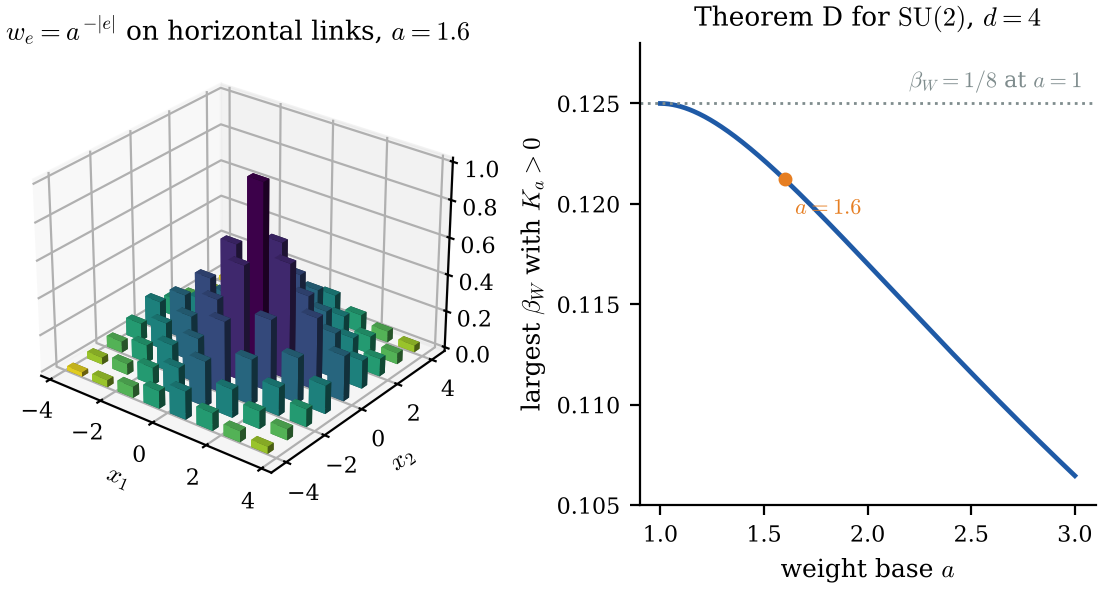
\includegraphics[width=0.96\textwidth]{figures/fig_weights.png}
\caption{The weights $w_e=a^{-|e|}$ of the distance~\eqref{eq:rhoa} on the
horizontal links of a $9\times9$ patch of $\Z^2$ (bar heights, $a=1.6$).
Links in a common plaquette have $\bigl||e|-|f|\bigr|\le1$, so the ratio
$w_e/w_f$ lies in $[a^{-1},a]$; the proof of Lemma~\ref{lem:weighted} pays
only $\frac12(r^{1/2}+r^{-1/2})-1\le(\sqrt a-1)^2/(2\sqrt a)$ for each such
ratio $r$, which vanishes as $a\to1$. Right: the largest $\beta_W$ for which
the constant $K_a$ of Theorem~D is positive, for four-dimensional $\SU(2)$; it
decreases from $1/8$ at $a=1$, and at $a=1.6$ it is $0.1212$.}
\label{fig:weights}
\end{figure*}

\section{SU(2): the single-link law}\label{sec:su2}

\subsection{The von Mises--Fisher law}

Identify $\SU(2)$ with the unit quaternions, that is with the unit sphere
$S^3\subset\R^4$, so that $\ReTr U=2x_0(U)$ and $\ReTr(UV)=2\ip u{\bar v}$
for the Euclidean inner product of $\R^4$ and quaternion conjugation
$v\mapsto\bar v$. Fix a link $e$ and the field off $e$. Every plaquette
through $e$ can be rotated cyclically so that its trace reads $\ReTr(Q_eA_p)$
with $A_p\in\SU(2)$, the staple of $e$ in $p$. The action therefore depends on
$Q_e$ only through
\[
N\beta\sum_{p\ni e}\ReTr(Q_eA_p)=\ip{x}{b},\qquad
b=4\beta\sum_{p\ni e}\bar A_p\in\R^4,
\]
with $x=Q_e\in S^3$. Since there are $2(d-1)$ staples, each of norm one,
\begin{equation}\label{eq:kappamax}
\kappa:=|b|\le y:=8(d-1)|\beta| .
\end{equation}
The conditional law of $Q_e$ is the von Mises--Fisher law\footnote{On the
sphere $S^{p-1}\subset\R^p$ the von Mises--Fisher law with mean direction
$\mu$ and concentration $\kappa$ has density proportional to
$e^{\kappa\ip x\mu}$ with respect to the surface measure, and its normalising
constant is $(2\pi)^{p/2}I_{p/2-1}(\kappa)/\kappa^{p/2-1}$; it is the maximum
entropy law with prescribed mean resultant, and it plays on the sphere the
role of the Gaussian in $\R^p$. For $p=4$ the Bessel index is $1$. The mean
resultant length $\E\ip x\mu=I_{p/2}(\kappa)/I_{p/2-1}(\kappa)$ is the
function $A$ of Lemma~\ref{lem:moments}. See Mardia and Jupp~\cite{MJ00},
Ch.~9, for these facts and for the tangent-normal decomposition used in
Appendix~\ref{app:vmf}.}
\begin{equation}\label{eq:vmf}
\nu_b(dx)=Z(\kappa)^{-1}e^{\ip xb}\,\sigma(dx)
\end{equation}
on the unit sphere, with $\sigma$ the normalised surface measure. We use
coordinates in which $b=\kappa e_1$. The density of $t=x_1$ is proportional
to $(1-t^2)^{1/2}e^{\kappa t}$ on $[-1,1]$, so $Z(\kappa)=2I_1(\kappa)/\kappa$
with the modified Bessel function $I_1$, normalised so that $Z(0)=1$.

\begin{lemma}\label{lem:vmf}
For every $\kappa\ge0$ the law $\nu_b$ on the unit sphere $S^3$ satisfies
the Poincar\'e inequality $\Var_{\nu_b}(g)\le\frac13\int|\nabla g|^2d\nu_b$,
and the constant $\frac13$ is attained at $\kappa=0$.
\end{lemma}

\begin{proof}
In the polar angle $\theta\in(0,\pi)$ from $e_1$ the generator of the
reversible diffusion of $\nu_b$ is $L=\partial_\theta^2+b(\theta)
\partial_\theta+\sin^{-2}\theta\,\Delta_{S^2}$ with $b(\theta)=2\cot\theta-
\kappa\sin\theta$. On spherical harmonics of degree $\ell$ on $S^2$ it acts as
a Sturm--Liouville operator $L_\ell$ with potential
$\ell(\ell+1)\sin^{-2}\theta$. A ground state comparison of Barta's
type~\cite{Bar37} with the trial function $\psi=\sin\theta\,
e^{a\kappa\cos\theta}$ gives $-L_1\psi\ge3\psi$ for $a=-\frac15$, and the same
trial function with $a=-\frac25$ gives the bound $3$ for the derivatives of
zonal eigenfunctions; Appendix~\ref{app:vmf} carries out both computations.
Hence every nonzero eigenvalue of $-L$ is at least $3$. At $\kappa=0$ the
first eigenvalue of the Laplacian of the unit $S^3$ is $3$.
\end{proof}

\subsection{Moments}

Let $A(\kappa)=\E_{\nu_b}x_1=Z'(\kappa)/Z(\kappa)=I_2(\kappa)/I_1(\kappa)$.

\begin{lemma}\label{lem:moments}
For every $\kappa>0$, in coordinates with $b=\kappa e_1$,
\begin{enumerate}[label=\textup{(\roman*)},leftmargin=*]
\item $\E x_2^2=\E x_3^2=\E x_4^2=A/\kappa$, $\E(1-x_1^2)=3A/\kappa$, the
covariance matrix of $x$ is $\operatorname{diag}(A',A/\kappa,A/\kappa,
A/\kappa)$, and $A'=1-A^2-3A/\kappa$;
\item $\displaystyle\frac{\kappa}{2+\sqrt{\kappa^2+4}}\le
A(\kappa)\le\frac{\kappa}{1+\sqrt{\kappa^2+9}}$;
\item $A'\le A/\kappa\le\bigl(1+\sqrt{\kappa^2+9}\bigr)^{-1}\le\frac14$.
\end{enumerate}
\end{lemma}

\begin{proof}
(i) Integrating by parts against $\frac{d}{dt}(1-t^2)^{3/2}=-3t(1-t^2)^{1/2}$
gives $\kappa\,\E(1-x_1^2)=3\E x_1$, and the three coordinates
$x_2,x_3,x_4$ are exchangeable under $\nu_b$, with $\sum_ix_i^2=1$. The
off-diagonal covariances vanish by the reflections $x_i\mapsto-x_i$,
$i\ge2$, and $A'=\Var x_1$ because $A=(\log Z)'$.
(ii) By (i), $A$ solves the Riccati equation $A'=1-A^2-3A/\kappa$ with
$A(\kappa)=\kappa/4+O(\kappa^3)$. Appendix~\ref{app:vmf} shows that the left
side of (ii) is a subsolution and the right side a supersolution of this
equation, with the same behaviour at $0$, and concludes by comparison.
(iii) The middle inequality is (ii). For the first, put $s=\sqrt{\kappa^2+4}$.
By (ii), $4A/\kappa\ge4/(2+s)$ and $1-A^2\le1-\kappa^2/(2+s)^2$, and
\[
\begin{aligned}
1-\frac{\kappa^2}{(2+s)^2}\le\frac4{2+s}
&\iff(2+s)^2-\kappa^2\le4(2+s)\\
&\iff s^2-\kappa^2\le4,
\end{aligned}
\]
which holds with equality. So $A'=1-A^2-3A/\kappa\le A/\kappa$.
\end{proof}

\subsection{The Lipschitz rate of the family}

Let $\delta$ be the chordal metric $\delta(x,x')=|x-x'|$ on $S^3$ and $W_1$
the Kantorovich distance for $\delta$. For $c\in\R^4$ and a unit vector
$h\in\R^4$ put
\begin{equation}\label{eq:rate}
L(c,h)=\sup_g\Cov_{\nu_c}\bigl(g,\ip hx\bigr),
\end{equation}
the supremum over $1$-Lipschitz functions $g$ for $\delta$. Since
$\frac{d}{dt}\nu_{c+th}(g)=\Cov_{\nu_{c+th}}(g,\ip hx)$, the
Kantorovich--Rubinstein duality gives, for all $b,b'$,
\begin{equation}\label{eq:w1segment}
W_1(\nu_b,\nu_{b'})\le|b-b'|\sup_{c\in[b,b']}L\Bigl(c,\frac{b'-b}{|b'-b|}
\Bigr).
\end{equation}
By rotation invariance $L(c,h)$ depends only on $\kappa=|c|$ and on the angle
$\varphi$ between $h$ and $c^\perp$, and we write $L(\kappa,\varphi)$.

\begin{lemma}\label{lem:rate}
For all $c$ and $h$, $L(c,h)\le1/(2\sqrt3)$. Moreover:
\begin{enumerate}[label=\textup{(\roman*)},leftmargin=*]
\item at $c=0$, $L(0,h)=\frac14$ for every $h$;
\item if $h\perp c$, then $L(c,h)=\E_{\nu_c}x_2^2=A(\kappa)/\kappa\le\frac14$;
\item if $\kappa\ge\sqrt{88}/3\approx3.127$, then $L(c,h)\le\frac14$ for
every $h$.
\end{enumerate}
\end{lemma}

\begin{proof}
A $1$-Lipschitz function for $\delta$ is $1$-Lipschitz for the geodesic
distance, which is larger, so $|\nabla g|\le1$ almost everywhere, and
Lemma~\ref{lem:vmf} gives $\Var g\le\frac13$. By Lemma~\ref{lem:moments}(i),
(iii) the largest eigenvalue of the covariance of $x$ is $A/\kappa\le\frac14$,
so $\Var\ip hx\le A/\kappa$. The Cauchy--Schwarz inequality gives
\begin{equation}\label{eq:csbound}
L(c,h)\le\bigl(\tfrac13A/\kappa\bigr)^{1/2}\le\Bigl(3\bigl(1+
\sqrt{\kappa^2+9}\bigr)\Bigr)^{-1/2}\le\frac1{2\sqrt3}.
\end{equation}
(i) and (ii) are reflection arguments. Let $R$ be the reflection in the
hyperplane $h^\perp$, and suppose $\nu_c$ is $R$-invariant, which is the case
when $c=0$ or $h\perp c$. Then $\E\ip hx=0$ and
\[
\begin{aligned}
\Cov(g,\ip hx)&=\E\bigl[(g(x)-g(Rx))\ip hx;\ \ip hx>0\bigr]\\
&\le\E\bigl[2\ip hx^2;\ \ip hx>0\bigr]=\E\ip hx^2,
\end{aligned}
\]
since $\delta(x,Rx)=2|\ip hx|$. Equality holds for $g=\ip hx$, which is
$1$-Lipschitz. At $c=0$, $\E\ip hx^2=\frac14$; for $h\perp c$, $\E\ip
hx^2=A/\kappa$. (iii) By~\eqref{eq:csbound}, $L\le\frac14$ as soon as
$1+\sqrt{\kappa^2+9}\ge\frac{16}3$, that is $\kappa^2\ge\frac{88}9$.
\end{proof}

The reflection is drawn in Fig.~\ref{fig:sphere}. Lemma~\ref{lem:rate}
leaves one case open, and Theorem~E would improve to the ceiling of
Proposition~\ref{prop:ceiling} if it were settled.

\begin{conjecture}[The sharp quarter]\label{conj:quarter}
$L(\kappa,\varphi)\le\frac14$ for all $\kappa\ge0$ and $\varphi$. By
Lemma~\ref{lem:rate} it suffices to take $0<\kappa<\sqrt{88}/3$ and
$\varphi<\pi/2$, and for Theorem~E at $\beta_W=2/9$ only $\kappa\le4/3$ is
needed.
\end{conjecture}

Figure~\ref{fig:surface} shows $L(\kappa,\varphi)$ computed by exact optimal
transport on a discretisation of $S^3$.\footnote{By symmetry the problem
reduces to the half two-sphere $\{(x_1,x_2,r):x_1^2+x_2^2+r^2=1,\ r\ge0\}$,
the quotient of $S^3$ by the rotations of the $(x_3,x_4)$ plane, with the
density $e^{\kappa x_1}r$ and the quotient metric, which is again the chordal
one. On a grid of $26\times26$ cells the computed values at $\kappa=0$ exceed
$\frac14$ by at most $5\times10^{-4}$, which is the discretisation error; at
$\varphi=\pi/2$ they agree with $A/\kappa$ to the same accuracy.} In every
computed case the maximum over $\varphi$ is at $\varphi=\pi/2$, where it equals
$A/\kappa$, and it decreases in $\kappa$. We have not been able to prove
this in general, but the question reduces to a variance inequality in two
variables.

\begin{proposition}[Reduction of the conjecture]\label{prop:reduction}
Let $c=\kappa e_1$, let $h$ lie in the plane of $e_1,e_2$, and let
$\mathcal L_{\rm sym}$ be the set of functions $g$ on $S^3$ that are
$1$-Lipschitz for $\delta$ and depend only on $(x_1,x_2,\sqrt{x_3^2+x_4^2})$.
Put $V(\kappa)=\sup_{g\in\mathcal L_{\rm sym}}\Var_{\nu_c}g$. Then
$V(\kappa)\ge A(\kappa)/\kappa$, and
\[
L(c,h)\le\bigl(V(\kappa)\,A(\kappa)/\kappa\bigr)^{1/2}.
\]
In particular, if linear functions maximise the variance in
$\mathcal L_{\rm sym}$, that is if $V(\kappa)=A(\kappa)/\kappa$, then
$L(\kappa,\varphi)\le A(\kappa)/\kappa\le\frac14$ for every $\varphi$, and
Conjecture~\ref{conj:quarter} holds with the maximum over $\varphi$ attained at
$\varphi=\pi/2$.
\end{proposition}

\begin{proof}
The group $H\cong\mathrm O(2)$ of orthogonal maps that fix $e_1$ and $e_2$
and act on the plane of $e_3,e_4$ preserves $\delta$, the law $\nu_c$ and the
function $\ip hx$. For a $1$-Lipschitz $g$ the average
$\bar g(x)=\int_Hg(kx)\,dk$ over the Haar measure of $H$ is again
$1$-Lipschitz, lies in $\mathcal L_{\rm sym}$, and has
$\Cov(\bar g,\ip hx)=\Cov(g,\ip hx)$. So the supremum in~\eqref{eq:rate} may
be taken over $\mathcal L_{\rm sym}$, and the Cauchy--Schwarz inequality with
$\Var\ip hx\le A/\kappa$ (Lemma~\ref{lem:moments}) gives the bound. The
function $x_2$ lies in $\mathcal L_{\rm sym}$ and has variance $A/\kappa$.
\end{proof}

The reduced problem lives on the upper half of the unit two-sphere in the
coordinates $(x_1,x_2,r)$, $r=(x_3^2+x_4^2)^{1/2}$, with the density
$r\,e^{\kappa x_1}$ and the chordal metric of $\R^3$, and asks whether a
linear function has the largest variance among all $1$-Lipschitz
functions.\footnote{The averaging step cannot be dropped: on all of $S^3$ the
maximal variance of a chordally $1$-Lipschitz function is not known to us,
and the Poincar\'e inequality of Lemma~\ref{lem:vmf} bounds it only by
$\frac13$, which is what leads to the constant $1/(2\sqrt3)$ of
Lemma~\ref{lem:rate}. In the geodesic metric the answer is different and
larger: at $\kappa=0$ the function $\arcsin x_2$ is geodesically $1$-Lipschitz
and has variance $\frac{\pi^2}{12}-\frac12\approx0.3225$, which exceeds
$\frac14$; its covariance with $x_2$ is $\frac8{9\pi}\approx0.283$, so in the
geodesic metric the rate at $\kappa=0$ is already larger than $\frac14$. The
chordal metric is therefore essential to the conjecture, and any proof must
see the curvature of the sphere at large distances, not only the length of
gradients.} For functions of $x_2$ alone the answer is yes: the condition
reads $|\psi(\alpha)-\psi(\alpha')|\le2\sin\frac{|\alpha-\alpha'|}2$ for
$\psi(\alpha)=g(\sin\alpha)$, and on a grid of $300$ angles the largest
variance found by linear programming at $\kappa=0$ is $\frac14$ to seven
digits. For general functions in $\mathcal L_{\rm sym}$ the same computation
on $450$ points of the half-sphere gives, at $\kappa=0,1,2$, the values
$0.25038$, $0.24056$, $0.21691$ against $A/\kappa=0.25000$, $0.24019$,
$0.21656$, differences of the size of the grid error. We do not have a proof.

\begin{figure*}[t]
\centering
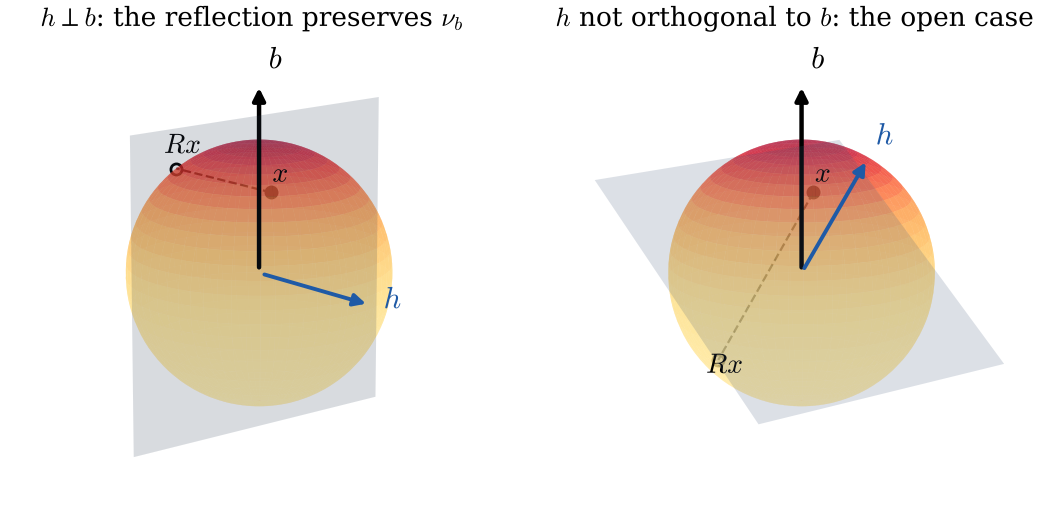
\includegraphics[width=0.96\textwidth]{figures/fig_sphere.png}
\caption{The single-link law on $S^3$, drawn in the three coordinates
$(x_1,x_2,x_3)$. Left: the von Mises--Fisher density for $\kappa=2$, peaked
in the staple direction $b$; the plane $h^\perp$ with $h\perp b$ and the
reflection $x\mapsto Rx$ that proves Lemma~\ref{lem:rate}(ii), which moves
each point by $2|\ip hx|$. Right: for $h$ not perpendicular to $b$ the
reflection no longer preserves the law, which is the open case of
Conjecture~\ref{conj:quarter}.}
\label{fig:sphere}
\end{figure*}

\begin{figure*}[t]
\centering
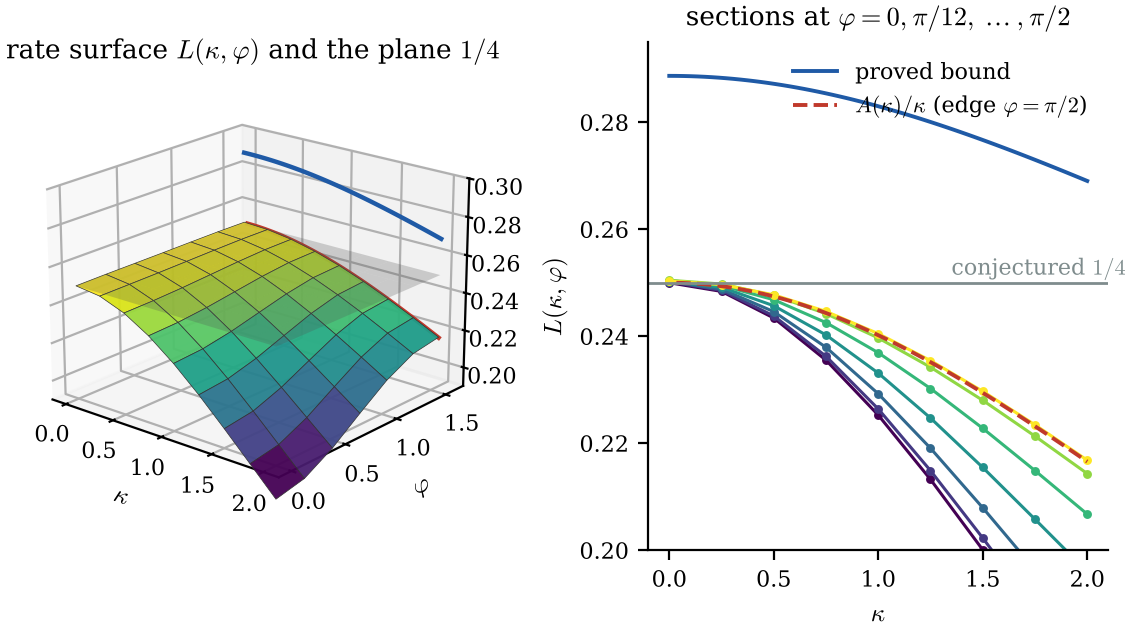
\includegraphics[width=0.96\textwidth]{figures/fig_surface.png}
\caption{The Lipschitz rate $L(\kappa,\varphi)$ of the von Mises--Fisher
family on $S^3$ (surface, computed by optimal transport), the conjectured
bound $\frac14$ (flat grey plane) and the proved bound
$(3(1+\sqrt{\kappa^2+9}))^{-1/2}$ of~\eqref{eq:csbound} (blue curve). The edge $\varphi=\pi/2$ is the proved value $A(\kappa)/\kappa$.
Right: sections at seven values of $\varphi$; for $\kappa\ge\frac12$ the
largest computed rate occurs at $\varphi=\pi/2$, where it is the proved
value. The
surface stays below the plane up to the discretisation error of the
transport computation, which shows at $\kappa=0$: there every direction
gives exactly $\frac14$ and the computed values exceed it by at most
$5\times10^{-4}$.}
\label{fig:surface}
\end{figure*}

\subsection{Proof of Theorem E}

\begin{proof}
For links $e\ne e'$ let
\[
C_{ee'}=\sup\frac{W_1\bigl(\gamma_e(\cdot\mid\omega),\gamma_e(\cdot\mid
\omega')\bigr)}{\delta(\omega_{e'},\omega'_{e'})},
\]
the supremum over pairs of fields that differ only at $e'$, where
$\gamma_e(\cdot\mid\omega)$ is the conditional law of $Q_e$. If $e$ and $e'$
do not share a plaquette, $C_{ee'}=0$. Otherwise they share exactly one
plaquette, and moving $Q_{e'}$ from $\omega_{e'}$ to $\omega'_{e'}$ changes
one staple of $e$ by an isometric image of the displacement, because left
and right multiplication by unit quaternions and conjugation are isometries
of $\R^4$. So $|b-b'|=4|\beta|\,\delta(\omega_{e'},\omega'_{e'})$, and
by~\eqref{eq:w1segment} and Lemma~\ref{lem:rate},
\[
C_{ee'}\le4|\beta|\cdot\frac1{2\sqrt3}=\frac{2|\beta|}{\sqrt3}.
\]
A link lies in $2(d-1)$ plaquettes, each with three other links, so every row
and every column of $C$ has at most $6(d-1)$ nonzero entries and
\[
\alpha:=\max\Bigl(\sup_e\sum_{e'}C_{ee'},\ \sup_{e'}\sum_eC_{ee'}\Bigr)\le4\sqrt3(d-1)|\beta| .
\]
For $\alpha<1$ the comparison lemma of Appendix~\ref{app:dobrushin}
(Lemma~\ref{lem:comparison}) gives uniqueness of the Gibbs measure and
decay of truncated correlations of Lipschitz local functions at every rate
$\lambda<-\log\alpha$, measured in the distance between link midpoints. At
$d=4$, $\alpha<1$ reads $|\beta|<1/(12\sqrt3)$, that is $\beta_W<1/(3\sqrt3)$.
\end{proof}

\begin{proposition}[The ceiling]\label{prop:ceiling}
Let $\delta$ be the chordal or the geodesic metric of $S^3$, used both at
$e'$ and for the Kantorovich distance at $e$. For all links $e,e'$ in a
common plaquette, $C_{ee'}\ge|\beta|$. Hence no argument through single-link
Dobrushin coefficients proves uniqueness beyond $|\beta|=1/(6(d-1))$.
\end{proposition}

\begin{proof}
The $2(d-1)$ staples of $e$ involve pairwise disjoint sets of links other
than $e'$, so they can be chosen with sum zero while the staple through $e'$
is arbitrary. Then $b=0$ and $\gamma_e$ is uniform. By
Lemma~\ref{lem:rate}(i) the derivative of $\nu_b$ at $b=0$ in the direction
$h$ has Kantorovich norm $\frac14|h|$ in the chordal metric, and at least
that in the geodesic one, tested against $\ip x{\hat h}$. With
$|b-b'|=4|\beta|\delta$ to first order this gives $C_{ee'}\ge|\beta|$, and
summing over the $6(d-1)$ neighbours gives $\alpha\ge6(d-1)|\beta|$.
\end{proof}

If Conjecture~\ref{conj:quarter} holds, the proof of Theorem~E gives
$C_{ee'}\le|\beta|$ and uniqueness for $|\beta|<1/(6(d-1))$, which is the
ceiling exactly.\footnote{A 2026 preprint attributed to J.~Lockwood, which we
have seen only as an abstract, announces uniqueness for four-dimensional
$\SU(2)$ at $\beta_W<2/9$ by a Wasserstein--Dobrushin argument. By
Proposition~\ref{prop:ceiling} that is the ceiling of the method, and it
would follow from Conjecture~\ref{conj:quarter}. We have not been able to
check the claim.} For $\SU(N)$ with $N\ge3$ the staple sum is not a multiple
of a unitary matrix, the single-link law is not of von Mises--Fisher type, and
the same argument with the single-link Bakry--\'Emery bound reproduces only
$|\beta|<1/(16(d-1))$; Theorem~D is stronger there.

\section{A gauge-invariant finite-box criterion}\label{sec:box}

\subsection{Interactions and boundary data}

Let $G$ be a compact metrisable group with normalised Haar measure $\lambda$,
and $E$ the set of positively oriented links of $\Z^d$ or of a torus. An
interaction is a family $\Phi=(\Phi_X)$ indexed by finite sets $X\subset E$ of
diameter at most $R$, with $\Phi_X\colon G^X\to\R$ continuous, invariant under
translations, and gauge invariant: $\Phi_X(gU)=\Phi_X(U)$ for every
$g\colon\Z^d\to G$, where $(gU)_{xy}=g_xU_{xy}g_y^{-1}$. The Wilson action is
$\Phi_p=-N\beta\ReTr U_p$; a renormalised effective action adds further
terms.\footnote{The definitions are written for the energy $\sum\Phi_X$ with
the Gibbs factor $e^{-\sum\Phi_X}$, which is the convention of the
probability literature; for the Wilson action this is the same measure as
in~\eqref{eq:wilson}.}

For finite $V\subset E$ let $\partial V=\bigcup\{X\setminus V:X\cap V\ne
\emptyset,\ \Phi_X\not\equiv0\}$. The specification is
\[
\gamma_V(dU_V\mid\omega)=Z_V(\omega)^{-1}e^{-\sum_{X\cap V\ne\emptyset}
\Phi_X(U_V\omega)}\lambda^V(dU_V),
\]
which depends on $\omega$ only through $\omega_{\partial V}$. Let $I(V)$ be the
set of vertices all of whose incident links lie in $V$, and
$\mathcal G_V=G^{I(V)}$. A gauge transformation at $x\in I(V)$ moves only links
of $V$, so
\begin{equation}\label{eq:interiorinv}
g_*\gamma_V(\cdot\mid\omega)=\gamma_V(\cdot\mid\omega)\qquad(g\in\mathcal
G_V).
\end{equation}

\begin{lemma}\label{lem:quotient}
Let $\Gamma_V$ be the graph with edge set $\partial V$. If
$\omega'_{\partial V}=(h\omega)_{\partial V}$ for a map $h$ from the vertices of
$\Gamma_V$ to $G$, then $\gamma_V(\cdot\mid\omega')=(\tilde h|_V)_*\gamma_V(
\cdot\mid\omega)$ for every extension $\tilde h$ of $h$. Consequently
gauge-invariant expectations $\gamma_V(F\mid\omega)$ depend only on the class of
$\omega_{\partial V}$ in $G^{\partial V}/G^{\mathrm{vert}(\Gamma_V)}$, which for
each connected component of $\Gamma_V$ is the space of holonomy
representations of its fundamental group modulo conjugation.
\end{lemma}

\begin{proof}
Change variables $U_V\mapsto\tilde hU_V$: Haar measure and the energy are
invariant. For the second statement, gauge the links of a spanning tree of
each component to the identity; the remaining links are free generators of
the fundamental group, and the residual freedom is one constant per
component, acting by conjugation.\footnote{This is the holonomy of a gauge
field on a graph; for holonomy in the Riemannian sense, in a related $\SU(n)$
setting, see~\cite{BTBS26}.}
\end{proof}

Plaquette holonomies alone do not determine this class when $G$ is
non-abelian; holonomies of larger loops of the shell enter.\footnote{Take two
plaquettes of the shell sharing a vertex, with based holonomies $(X,Y)$ and
$(X,Y')$, where $X=Y=\mathrm i\sigma_3$ and $Y'=\mathrm i\sigma_1$ in
$\SU(2)$. Each holonomy is conjugate to its partner, but $\Tr(XY)=-2\ne0=
\Tr(XY')$, and $XY$ is the holonomy of the boundary of the union of the two
plaquettes.} The criterion below therefore compares boundary conditions that
differ at one link.

\begin{lemma}[Gauge lift]\label{lem:lift}
Let $\Pi$ be a coupling of $\gamma_V(\cdot\mid\omega)$ and
$\gamma_V(\cdot\mid\omega')$, let $g\colon G^V\times G^V\to\mathcal G_V$ be
measurable, and let $h$ be Haar distributed on $\mathcal G_V$, independent of
$(U,U')\sim\Pi$. Then $(hU,\,hg(U,U')U')$ is again a coupling of the two
measures, and $\mathbb P[(hU)_b\ne(hgU')_b]=\Pi[U_b\ne(g(U,U')U')_b]$ for
every link $b$.
\end{lemma}

\begin{proof}
By~\eqref{eq:interiorinv}, $hU\sim\gamma_V(\cdot\mid\omega)$. Given $(U,U')$
the element $hg$ is Haar distributed, so $hgU'$ is uniform on the
$\mathcal G_V$-orbit of $U'$, and by~\eqref{eq:interiorinv} again
$hgU'\sim\gamma_V(\cdot\mid\omega')$. Each $h_x$ acts on a link by a bijection
of $G$, which preserves equality of the two link values.
\end{proof}

\subsection{The criterion}

Write $V_\mu$ for the links of $V$ in direction $\mu$, $n_{\min}=\min_\mu
|V_\mu|$, and $\omega\sim_y\omega'$ when $\omega,\omega'$ differ only at the
link $y\in\partial V$.

\begin{definition}\label{def:gds}
The interaction satisfies the gauge Dobrushin--Shlosman condition
$\mathrm{GDS}(V,\varepsilon)$ if there are a Borel family of couplings
$\Pi_{\omega,\omega'}$ of $\gamma_V(\cdot\mid\omega)$ and
$\gamma_V(\cdot\mid\omega')$, for all pairs $\omega\sim_y\omega'$, and numbers
$\kappa_V(y,b)\ge\sup_{\omega\sim_y\omega'}\Pi_{\omega,\omega'}[U_b\ne
U'_b]$ for $y\in\partial V$, $b\in V$, such that for every direction $\nu$
\begin{equation}\label{eq:gds}
K_V(\nu):=\sum_{y\in\partial V,\ \mathrm{dir}\,y=\nu}\ \sum_{b\in V}
\kappa_V(y,b)\ \le\ (1-\varepsilon)\,n_{\min}.
\end{equation}
\end{definition}

By Lemmas~\ref{lem:quotient} and~\ref{lem:lift} the couplings may be built on
the gauge quotient and then aligned by any measurable choice of interior
gauge, and the supremum is a supremum over classes of shell holonomies
(Fig.~\ref{fig:box}). For a box symmetric under the hypercubic group,
\eqref{eq:gds} reads $\sum_{y,b}\kappa_V(y,b)\le(1-\varepsilon)|V|$, the form
of Dobrushin and Shlosman~\cite{DS85}, except that the supremum over boundary
conditions is taken for each $b$ separately; this is what makes the proof
below work for an arbitrary compact group.

\begin{theorem}\label{thm:box}
Assume $\mathrm{GDS}(V,\varepsilon)$ for a finite-range gauge-invariant
interaction with compact $G$. Let $D=\max\{|b-y|:b\in V,\ y\in\partial V\}$,
with distances between link midpoints, and $0<\lambda<|\log(1-\varepsilon)|
/D$, so that $\theta:=(1-\varepsilon)e^{\lambda D}<1$. Then:
\begin{enumerate}[label=\textup{(\roman*)},leftmargin=*]
\item There is exactly one Gibbs measure $\mu$ on $G^E$; it is invariant
under translations and gauge transformations.
\item Let $S\subset E$ be finite and $\mu_1,\mu_2$ probability measures
invariant under $\gamma_{V+a}$ for every translate with $(V+a)\cap
S=\emptyset$. Let $N_S$ be $S$ together with the links of the translates of
$V$ that meet $S$; then $|N_S|\le c_V|S|$. There is a coupling of $\mu_1$ and
$\mu_2$ under which, for every link $b$ at distance greater than $\diam V+R$
from $S$,
\[
\mathbb P[\sigma_b\ne\sigma'_b]\le\frac{\theta}{1-\theta}\sum_{z\in N_S}
e^{-\lambda|b-z|}.
\]
\item For bounded functions $F$ and $H$ with finite supports $S_F$ and
$S_H$, the covariance $|\Cov_\mu(F,H)|$ is at most
\[
2\|F\|_\infty\|H\|_\infty\frac{\theta c_V}{1-\theta}
|S_F||S_H|\,e^{-\lambda(\dist(S_F,S_H)-\diam V-R)} .
\]
\item Items \textup{(i)--(iii)} hold on every torus of side greater than
$2(\diam V+R)$ with the same constants, for the untwisted and for every
't~Hooft twisted Wilson action.
\end{enumerate}
\end{theorem}

\begin{proof}
\emph{A minimal coupling.} Let $W$ be $E$ or $E\setminus S$, let
$\mathcal A=\{a:V+a\subseteq W\}$ and $V_a=V+a$. Fix a link $b_0$ and put
$w_b=e^{-\lambda|b-b_0|}$, so that $\sum_bw_b<\infty$. On the set $\mathcal C$
of couplings of $\mu_1,\mu_2$ let $\Psi(\pi)=\sum_bw_b\,\pi[\sigma_b\ne
\sigma'_b]$. The set $\mathcal C$ is weakly compact because $G^E$ is compact,
and each map $\pi\mapsto\pi[\sigma_b\ne\sigma'_b]$ is lower semicontinuous,
being the measure of an open set. So $\Psi$ attains its minimum at some
$\pi^*$. Put $\rho(b)=\pi^*[\sigma_b\ne\sigma'_b]$.

\emph{Block resampling.} For $a\in\mathcal A$ define a new coupling $T_a\pi^*$:
sample $(\sigma,\sigma')\sim\pi^*$, keep both fields off $V_a$, and inside
$V_a$ sample from the following path coupling of $\gamma_{V_a}(\cdot\mid
\sigma)$ and $\gamma_{V_a}(\cdot\mid\sigma')$. List $\partial V_a=\{z_1,
\dots,z_k\}$ and let $\omega^j$ agree with $\sigma'$ on $z_1,\dots,z_j$ and
with $\sigma$ elsewhere. Consecutive $\omega^{j-1},\omega^j$ are equal or
differ only at $z_j$; couple their block laws by the identity in the first
case and by the translate of $\Pi_{\omega^{j-1},\omega^j}$ in the second, and
chain the couplings through their disintegrations, which depend measurably
on the parameters~\cite[Ch.~3]{Kal21}. This gives $\tau^0,\dots,\tau^k$ with
$\tau^0\sim\gamma_{V_a}(\cdot\mid\sigma)$, $\tau^k\sim\gamma_{V_a}(\cdot\mid
\sigma')$ and $\mathbf 1[\tau^0_b\ne\tau^k_b]\le\sum_j\mathbf 1[\tau^{j-1}_b
\ne\tau^j_b]$. Since each $\mu_i$ is $\gamma_{V_a}$-invariant,
$T_a\pi^*\in\mathcal C$, and for $b\in V_a$
\[
T_a\pi^*[\tau_b\ne\tau'_b]\le\sum_{z\in\partial V_a}\kappa_V(z-a,b-a)\rho(z),
\]
while nothing changes off $V_a$. Minimality, $\Psi(T_a\pi^*)\ge\Psi(\pi^*)$,
gives
\begin{equation}\label{eq:blockineq}
\sum_{b\in V_a}w_b\rho(b)\le\sum_{b\in V_a}w_b\sum_{z\in\partial V_a}
\kappa_V(z-a,b-a)\rho(z).
\end{equation}

\emph{Summation over blocks.} Sum~\eqref{eq:blockineq} over $a\in\mathcal A$;
all series converge, the left side being at most $|V|\sum_bw_b$. Let $W^\circ$
be the set of links $b$ such that every translate of $V$ containing $b$ lies
in $W$; then $E\setminus W^\circ\subseteq N_S$. A link $b$ of direction $\mu$
lies in exactly $|V_\mu|\ge n_{\min}$ translates. On the right, $|z-b|\le D$
gives $w_b\le e^{\lambda D}w_z$, and for fixed $z$ of direction $\nu$ the sum
over all $a$ with $z\in\partial V_a$ and all $b\in V_a$ of $\kappa_V(z-a,b-a)$
equals $K_V(\nu)$. By~\eqref{eq:gds},
\[
n_{\min}\sum_{b\in W^\circ}w_b\rho(b)\le\theta\,n_{\min}\Bigl[\sum_{z\in
W^\circ}w_z\rho(z)+\sum_{z\in N_S}w_z\Bigr],
\]
so $\sum_{W^\circ}w\rho\le\frac{\theta}{1-\theta}\sum_{z\in N_S}w_z$. Taking
$b_0\in W^\circ$ and keeping only the term $b=b_0$ on the left proves (ii).

\emph{Uniqueness.} With $S=\emptyset$, $N_S=\emptyset$ and $\rho\equiv0$, so
any two Gibbs measures coincide. Gibbs measures exist by compactness, and
translates and gauge transforms of a Gibbs measure are Gibbs measures; since
there is only one, it is invariant. This is (i).

\emph{Decay.} Let $\mu^u=\mu(\cdot\mid U_{S_H}=u)$ be a regular conditional
probability; for $\mu$-almost every $u$ it is invariant under every
$\gamma_{V_a}$ with $V_a\cap S_H=\emptyset$. Since $\Cov(F,H)=\int H(u)
[\mu^u(F)-\int\mu^{u'}(F)\mu(du')]\mu(du)$, we get
$|\Cov(F,H)|\le\|H\|_\infty\operatorname{ess\,sup}_{u,u'}|\mu^u(F)-
\mu^{u'}(F)|$, and $|\mu^u(F)-\mu^{u'}(F)|\le2\|F\|_\infty\sum_{b\in S_F}
\rho(b)$. Item (ii) with $S=S_H$ gives (iii).

\emph{Tori and twists.} On a torus of side greater than $2(\diam V+R)$ every
translate is a genuine block and the argument is unchanged. Let $z_p\in Z(G)$
be a twist that is closed, so that on every ball of radius at least $\diam
V+R$ it equals $(dn)_p=\prod_{e\in\partial p}n_e^{\pm1}$ for some $n\colon E\to
Z(G)$; every 't~Hooft twist has this property, because a closed
$Z(G)$-valued $2$-cocycle is exact on a contractible ball. Multiplication
$M_n$ of each link by the central element $n_e$ satisfies
$\gamma^{\rm tw}_{V_a}(\cdot\mid\omega)=(M_n)_*\gamma_{V_a}(\cdot\mid
M_n\omega)$ on such a ball, since central factors commute through, and $M_n$
is a bijection on each link. So the twisted specification satisfies
$\mathrm{GDS}(V,\varepsilon)$ with the same $\kappa_V$. This is (iv).
\end{proof}

\begin{figure*}[t]
\centering
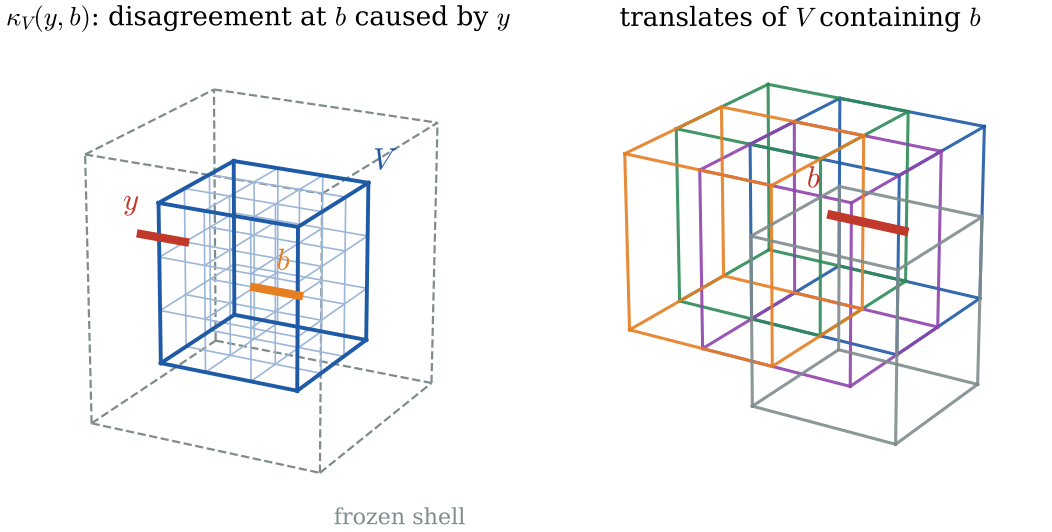
\includegraphics[width=0.96\textwidth]{figures/fig_box.png}
\caption{The finite-box criterion. Left: a box $V$ inside its frozen shell
and a boundary link $y$; two copies of the box are coupled with boundary
conditions that differ only at $y$, and $\kappa_V(y,b)$ bounds the chance
that they disagree at $b$ after the best interior gauge alignment. Right:
the translates of $V$ covering a link $b$; the proof of
Theorem~\ref{thm:box} resamples one translate at a time and sums the
resulting inequalities.}
\label{fig:box}
\end{figure*}

\subsection{Confinement and stability}

Let $\mathcal V$ be the family of sets $V\cap W'$, where $W'$ runs over the
interior link sets of all cubes in all positions. The box-hereditary
condition $\mathrm{HGDS}(V,\varepsilon)$ is~\eqref{eq:gds} with
$\sum_b\kappa_V(y,b)$ replaced by $\sup_{V'\in\mathcal V,\ y\in\partial V'}
\sum_{b\in V'}\kappa_{V'}(y,b)$, the boundary condition of $V'$ including the
links of $V\setminus V'$.

\begin{proposition}\label{prop:hgds}
Assume $\mathrm{HGDS}(V,\varepsilon)$ for the Wilson action of a compact
group $G\subset\U(n)$. Then covariances of local functions under the
finite-volume measure of every cube with every boundary condition decay
exponentially, with constants independent of the cube and the boundary
condition. By Chatterjee's theorem~\cite[Thm.~2.4]{Cha21} the centre
symmetry is unbroken and, if the representation acts nontrivially on the
centre, Wilson loops obey the area law.
\end{proposition}

\begin{proof}
Fix a cube $B$ with boundary condition $\delta$, interior link set $W_B$, and
local functions $F,H$. Condition $\mu_{B,\delta}$ on $U_{S_H}=u$ and on
$U_{S_H}=u'$, and run the proof of Theorem~\ref{thm:box} in
$W=W_B\setminus S_H$ with all blocks $V_a\cap W_B$ that meet $W$. A link of
$W$ of direction $\mu$ lies in $|V_\mu|\ge n_{\min}$ blocks, so no boundary
layer is lost on the left of the summed inequality. A link $z\in W$ in
$\partial(V_a\cap W_B)$ lies in $\partial V_a$, and its total weight on the
right is bounded by the hereditary condition. The other links of
$\partial(V_a\cap W_B)$ lie outside $B$, where both copies carry $\delta$, or in
$S_H$. So the only sources of disagreement are the links of $S_H$, each with
weight at most $e^{\lambda D}(|V|+|\partial V|)|V|/n_{\min}$, and the bound
follows as in Theorem~\ref{thm:box}(iii), uniformly in $B$ and $\delta$. This
is the decay property of~\cite[Def.~2.3]{Cha21}.
\end{proof}

\begin{lemma}\label{lem:stability}
Suppose $\Phi$ satisfies $\mathrm{GDS}(V,\varepsilon)$ and $\Phi'=\Phi+
\mathcal E$ with $\mathcal E$ gauge invariant of range at most $R$. Put
$t=\tanh\bigl(\frac12\sum_{X\cap V\ne\emptyset}\|\mathcal E_X\|_\infty\bigr)$.
Then $\Phi'$ satisfies $\mathrm{GDS}(V,\varepsilon')$ with
$\varepsilon'=\varepsilon-2t|V|\max_\nu|\partial V|_\nu/n_{\min}$, where
$|\partial V|_\nu$ is the number of links of direction $\nu$ in $\partial V$.
\end{lemma}

\begin{proof}
The two energies on $V$ differ by a function of oscillation at most
$s=2\sum_{X\cap V\ne\emptyset}\|\mathcal E_X\|_\infty$, and two probability
measures whose log-densities differ by a function of oscillation $s$ are
within total variation $\tanh(s/4)$ (Lemma~\ref{lem:tanh}). Glue an optimal
coupling of $\gamma'_V(\cdot\mid\omega)$ with $\gamma_V(\cdot\mid\omega)$,
then $\Pi_{\omega,\omega'}$, then an optimal coupling of
$\gamma_V(\cdot\mid\omega')$ with $\gamma'_V(\cdot\mid\omega')$. Then
$\kappa'(y,b)\le\kappa(y,b)+2t$, and summing over $b\in V$ and over $y$ of
direction $\nu$ gives the stated loss.
\end{proof}

The smallness required in Lemma~\ref{lem:stability} shrinks with the box,
since $t$ must be of order $\varepsilon/(|V||\partial V|)$. This matters in
Sec.~\ref{sec:open}.

\subsection{Two dimensions}

In two dimensions the criterion holds at every coupling. Take $G=\SU(2)$ and
the plaquette weight $w(U)=e^{\frac\beta2\Tr U}$, write $c_0=\int w$,
$f=w/c_0$ and $a_j=I_{2j+1}(\beta)/I_1(\beta)$ for $j=\frac12,1,\dots$. The
character expansion of Appendix~\ref{app:twod} gives
$f^{*m}=\sum_j(2j+1)a_j^m\chi_j$ and
\[
\varepsilon_m:=\sup_U|f^{*m}(U)-1|=\sum_{j\ge1/2}(2j+1)^2a_j^m,
\]
which tends to $0$ exponentially as $m\to\infty$.

\begin{lemma}[Disk integration~\cite{Mig75,Lev03}]\label{lem:disk}
For a rectangle $D$ made of $k$ plaquettes,
$\int\prod_{p\subset D}w(U_p)\,dU_{\mathrm{int}\,D}=c_0^kf^{*k}(\mathrm{hol}_{
\partial D})$.
\end{lemma}

The proof is in Appendix~\ref{app:twod}.

\begin{proposition}\label{prop:2d}
For every $\beta>0$ there is $L$ such that two-dimensional $\SU(2)$ Wilson
theory satisfies $\mathrm{GDS}(V,\varepsilon)$ for the set $V$ of the
$2L(L-1)$ interior links of an $L\times L$ square and some $\varepsilon>0$.
\end{proposition}

\begin{proof}
For $y\in\partial V$ choose an $s\times s$ sub-square $D$ with $y$ on its
outer side; let $L_D$ be its $2s(s-1)$ interior links and $L_R=V\setminus
L_D$. By Lemma~\ref{lem:disk}, under $\gamma_V(\cdot\mid\omega)$ the marginal on
$L_R$ has density proportional to $\prod_{p\not\subset D}w(U_p)\cdot
f^{*s^2}(\mathrm{hol}_{\partial D})$, and only the last factor depends on
$\omega_y$. Two densities proportional to $\varrho g_1$ and $\varrho g_2$ with
$g_i\in[1-\epsilon,1+\epsilon]$ are within total variation
$\eta=2\epsilon/(1-\epsilon^2)$ (Appendix~\ref{app:twod}). Couple the two
marginals on $L_R$ maximally and sample $L_D$ independently; then
$\kappa(y,b)\le1$ on $L_D$ and $\kappa(y,b)\le\eta_{s^2}$ on $L_R$, with
$\eta_m=2\varepsilon_m/(1-\varepsilon_m^2)$. Since $|\partial V|_\nu=2L$ for
each direction and $n_{\min}=L(L-1)$, the condition~\eqref{eq:gds} holds when
$2L\bigl[2s(s-1)+2L(L-1)\eta_{s^2}\bigr]<L(L-1)$, that is
\[
\frac{4s(s-1)}{L-1}+4L\,\eta_{s^2}<1 .
\]
Choose $s$ with $\eta_{s^2}<1/(80s^2)$, which is possible because
$\eta_{s^2}$ decays exponentially in $s^2$, and then $L=8s^2$. Both terms are
then at most $\frac12-\frac1{80}$.
\end{proof}

In four-dimensional $\U(1)$ theory at large $\beta$ correlations decay only
as a power~\cite{Gut80,FS82}, so by Theorem~\ref{thm:box} no box satisfies
$\mathrm{GDS}$ there.\footnote{A weaker hypothesis, bounding only the
influence of one boundary link on one observable at the centre of the box,
would be met by the massless spin-wave part of that theory for large boxes,
since that influence decays like the fourth power of the box size. Such a
hypothesis cannot imply decay. The criterion has to measure joint couplings
of the whole box, as Definition~\ref{def:gds} does.}

\section{Transfer matrices and the mass gap}\label{sec:transfer}

In this section $d=4$ and $G\subset\U(N)$ is compact. Let $\Lambda_L=
(\Z/L\Z)^3$ be the spatial torus, with $3L^3$ links and $3L^3$ plaquettes,
$\mu$ the Haar measure on $G^{E_L}$ and $\mathcal H_L=L^2(G^{E_L},\mu)$. In
temporal gauge the Wilson measure~\eqref{eq:wilson} on $\Lambda_L\times\Z/T\Z$
equals $\Tr(\mathbb T_L^T)/Z$ for the integral operator with kernel
\begin{multline*}
k(U,V)=e^{\frac{N\beta}2\sum_p(\ReTr U_p+\ReTr V_p)}\\
\times\int_{G^{\Lambda_L}}\prod_{e=(x,y)}e^{N\beta\ReTr(U_eh_yV_e^{-1}
h_x^{-1})}\prod_xdh_x ,
\end{multline*}
the integral over $h$ being the integral over the timelike links. This is
the transfer matrix of Osterwalder and Seiler~\cite{OSei78}.\footnote{The
kernel is a positive operator because the Wilson action is reflection
positive for reflections in planes between lattice hyperplanes: the weight
splits as $F\cdot\Theta F$ times a factor $e^{N\beta\ReTr(U\,\Theta U)}$ on
the crossing plaquettes, and $\ReTr$ of a product of a matrix and its
reflection expands into a positive combination of products of a function and
its reflection, by the character expansion with nonnegative coefficients for
$\beta\ge0$. Reflection positivity in the time direction gives a Hilbert
space by the Osterwalder--Schrader construction~\cite{OS73,OS75}, and the
transfer matrix is the operator implementing one step of Euclidean time.
Brydges, Fr\"ohlich and Seiler~\cite{BFS79} developed this framework for
gauge fields, including gauge fixing and the identification of physical
states, as the starting point of a construction of the continuum theory; the
renormalisation group methods needed to continue from there are surveyed by
Rivasseau~\cite{Riv91}.}

\begin{proposition}[Finite-volume gap]\label{prop:finitegap}
For $\beta\ge0$ the operator $\mathbb T_L$ is self-adjoint, nonnegative,
Hilbert--Schmidt and positivity improving. Its largest eigenvalue
$\lambda_0$ is simple with a strictly positive eigenfunction, and every other
spectral value $\lambda$ satisfies $|\lambda|\le(1-e^{-12N^2\beta L^3})
\lambda_0$.
\end{proposition}

\begin{proof}
The kernel is continuous on a compact space, hence Hilbert--Schmidt, and
symmetric (substitute $h\mapsto h^{-1}$). Write $\mathbb T_L=A\mathcal K\Pi A$,
with $A$ multiplication by $e^{\frac{N\beta}2\sum_p\ReTr U_p}$, $\mathcal K$
the convolution on each link by $\kappa(g)=e^{N\beta\ReTr g}$, and $\Pi$ the
average over gauge transformations. Since $\ReTr g=\frac12(\chi_F(g)+
\overline{\chi_F(g)})$ and products of characters decompose with nonnegative
multiplicities, $\kappa$ has nonnegative character coefficients, so convolution
by it is a nonnegative operator; $\Pi$ is an orthogonal projection commuting
with $\mathcal K$, since $\kappa$ is a class function, so $\mathcal K\Pi=
\Pi\mathcal K\Pi\ge0$ and $\mathbb T_L\ge0$. From $|\ReTr g|\le N$,
\[
m_L:=e^{-6N^2\beta L^3}\le k(U,V)\le e^{6N^2\beta L^3}=:M_L,
\]
so $\mathbb T_L$ is positivity improving. By Jentzsch's
theorem~\cite{Jen12} $\lambda_0=\|\mathbb T_L\|$ is simple with an almost
everywhere positive eigenfunction $\psi_0$, and
$m_L\|\psi_0\|_1\le\lambda_0\psi_0\le M_L\|\psi_0\|_1$. The kernel
$p(U,V)=k(U,V)\psi_0(V)/(\lambda_0\psi_0(U))$ is Markov, reversible for
$\pi=\psi_0^2\mu/\|\psi_0\|_2^2$, and unitarily equivalent to
$\mathbb T_L/\lambda_0$. It satisfies $p(U,V)\ge\epsilon\psi_0(V)/
\|\psi_0\|_1$ with $\epsilon=m_L/M_L$, so by Doeblin's argument
$\|P^nf\|_\infty\le2(1-\epsilon)^n\|f\|_\infty$ for bounded $f$ with $\pi(f)=0$.
For the spectral measure $\sigma_f$ of $P$ at such $f$ this gives
$\int\lambda^{2n}d\sigma_f\le4(1-\epsilon)^{2n}\|f\|_\infty^2$ for all $n$, so
$\sigma_f$ vanishes on $\{|\lambda|>1-\epsilon\}$. Bounded mean-zero functions
are dense in the mean-zero subspace of $L^2(\pi)$.
\end{proof}

This holds for $\U(1)$ as well and carries no information about infinite
volume.\footnote{The bound $1-e^{-12N^2\beta L^3}$ tends to $1$ as
$L\to\infty$, so the finite-volume gap it gives tends to $0$; the content of a
mass gap is the uniformity in $L$, Proposition~\ref{prop:uniform}.}

Let $\omega$ be a state on the gauge-invariant local functions of $\Z^4$ that
is invariant under translations and the hypercubic group and reflection
positive for reflections in planes through sites and in planes bisecting
links. Every limit of Wilson states on periodic tori has these
properties~\cite{OSei78}. The reconstruction gives a Hilbert space with a
vector $\Omega$, a map $F\mapsto\Psi_F$ with dense range, and a self-adjoint
$\mathbb T$ with $0\le\mathbb T\le1$, $\mathbb T\Omega=\Omega$ and
$\ip{\Psi_F}{\mathbb T^t\Psi_H}=\omega(\vartheta(\bar F)\tau_tH)$, where
$\vartheta$ is the time reflection and $\tau_t$ the time
translation.\footnote{$\Psi_F$ is the class of $F$ in the completion of the
positive-time local functions for the form $\ip FH=\omega(\vartheta(\bar F)H)$,
which is positive semidefinite by reflection positivity. Since
$|\omega(\vartheta(\bar F)F)|\le\omega(|F|^2)$ by the Cauchy--Schwarz
inequality and the invariance of $\omega$ under $\vartheta$, functions that are
close in $L^2(\omega)$ give close vectors.}

\begin{proposition}\label{prop:gapdecay}
For $m>0$ the following are equivalent:
\begin{enumerate}[label=\textup{(\alph*)},leftmargin=*]
\item the spectrum of $\mathbb T$ on $\Omega^\perp$ lies in $[0,e^{-m}]$;
\item for every $F$ in a class of gauge-invariant local functions supported
at times in a bounded interval and dense in $L^2(\omega)$ on each such support,
there is $C_F<\infty$ with $0\le\omega(\vartheta(\bar F)\tau_tF)-|\omega(F)|^2
\le C_Fe^{-mt}$ for all $t\ge0$.
\end{enumerate}
Under \textup{(a)} one may take $C_F=\|F\|_\infty^2$ for every bounded $F$.
\end{proposition}

\begin{proof}
If (a) holds, then
\[
\omega(\vartheta(\bar F)\tau_tF)-|\omega(F)|^2=\ip{\Psi'_F}{\mathbb
T^t\Psi'_F}
\]
with $\Psi'_F=\Psi_F-\ip\Omega{\Psi_F}\Omega\in\Omega^\perp$; this number lies
in $[0,e^{-mt}\|\Psi_F\|^2]$, and $\|\Psi_F\|^2\le\|F\|_\infty^2$.
Conversely, let $\sigma$ be the spectral measure of $\mathbb T$ at
$\Psi'_F$ and let $\delta>0$. Then
\[
\sigma\bigl((e^{-m+\delta},1]\bigr)e^{(-m+\delta)t}\le C_Fe^{-mt}
\]
for all $t$, so $\sigma((e^{-m+\delta},1])=0$.
The spectral projection of $(e^{-m},1]$ restricted to $\Omega^\perp$ therefore
annihilates the vectors $\Psi'_F$ of the class, which are dense by the
footnote above, and it vanishes.
\end{proof}

Let $\Delta_L(\beta)=\log(\lambda_0/\lambda_1)$ be the gap of $\mathbb T_L$ and
$\omega_L$ its vacuum state.

\begin{proposition}\label{prop:uniform}
Let $m=\inf_L\Delta_L(\beta)$ and assume $m>0$. Then every weak limit
point $\omega$ of the sequence $(\omega_L)$ satisfies
\[
|\omega(F\tau_tH)-\omega(F)\omega(H)|\le\|F\|_\infty\|H\|_\infty e^{-mt}
\]
for gauge-invariant $F$ and $H$ on single time slices, and hence has
transfer-matrix gap at least $m$.
\end{proposition}

\begin{proof}
The truncated correlation $\omega_L(F\tau_tH)-\omega_L(F)\omega_L(H)$ equals
\[
\bigl\langle\bar F\Omega_L,(\mathbb T_L/\lambda_0)^t(1-|\Omega_L\rangle
\langle\Omega_L|)H\Omega_L\bigr\rangle,
\]
which is bounded by $\|F\|_\infty\|H\|_\infty
e^{-\Delta_Lt}$. The bound is uniform in $L$ and passes to weak limits, which
exist by compactness. Proposition~\ref{prop:gapdecay} completes the proof.
\end{proof}

\subsection{Proof of Theorem F}

\begin{proof}
\emph{The curvature range.} By Theorem~D the torus Wilson measures converge
to a single measure $\mu$, which is therefore translation and hypercubic
invariant and reflection positive, reflection positivity of each torus
measure~\cite{OSei78} being preserved under weak limits of local
expectations. By Theorem~B, smooth local functions have exponentially
decaying truncated correlations under $\mu$: for $F,H$ smooth and local,
$|\Cov_\mu(F,H)|\le C_{F,H}e^{-c\,\dist(\operatorname{supp}F,
\operatorname{supp}H)}$ with $c>0$~\cite[Cor.~4.11]{SZZ23}. Apply this to $F$
supported at times in $[0,s]$ and to $\vartheta(\bar F)$ and $\tau_tF$, whose
supports are at distance at least $t-1$. Smooth gauge-invariant local
functions with support in a fixed set are dense in $L^2(\mu)$ on that set
(average a smooth approximant over the compact gauge group of the support).
Proposition~\ref{prop:gapdecay} gives a gap $m\ge c$.

\emph{$\SU(2)$.} In the range of Theorem~E, every limit point of the
periodic torus measures is a Gibbs measure for the infinite-volume
specification~\cite[Ch.~4]{Geo11}, so it equals the unique Gibbs measure $\mu$,
which is again reflection positive. Lemma~\ref{lem:comparison} gives, for
local functions $F,H$ that are Lipschitz in each link variable,
$|\Cov_\mu(F,H)|\le C_{F,H}e^{-\lambda\,\dist(S_F,S_H)}$ for every
$\lambda<-\log\alpha$, with $\alpha=4\sqrt3(d-1)|\beta|$. Lipschitz
gauge-invariant local functions are dense as before, and
Proposition~\ref{prop:gapdecay} gives a gap at least $\lambda$ for each such
$\lambda$, hence at least $-\log\alpha$. At $d=4$, $\alpha=12\sqrt3|\beta|=
3\sqrt3\,\beta_W$.
\end{proof}

\begin{figure*}[t]
\centering
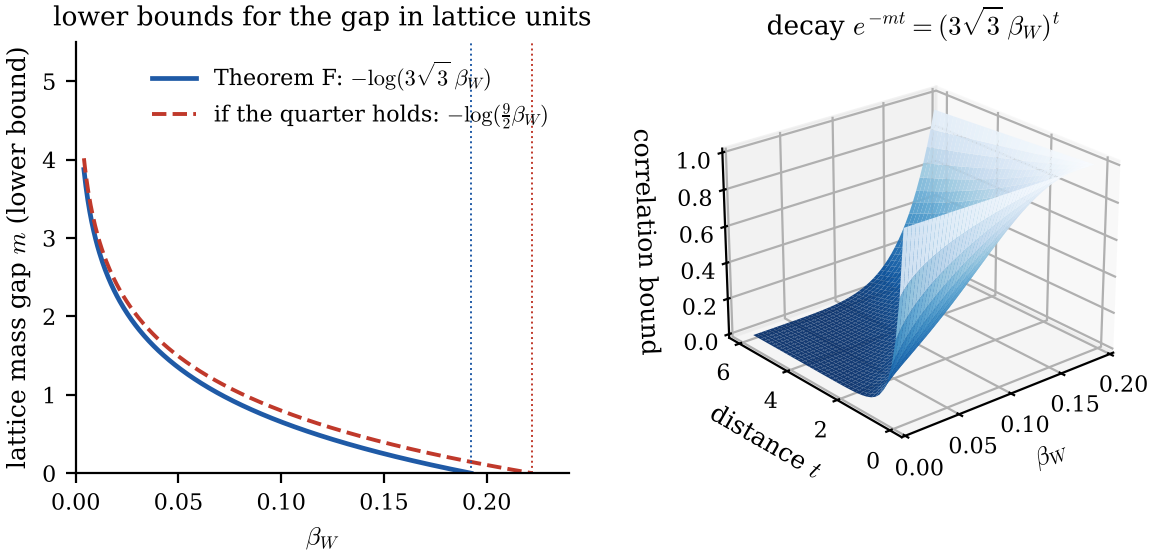
\includegraphics[width=0.96\textwidth]{figures/fig_massgap.png}
\caption{The lower bound $m\ge-\log(3\sqrt3\,\beta_W)$ of Theorem~F for
four-dimensional $\SU(2)$, in lattice units (solid), and the bound
$m\ge-\log(\frac92\beta_W)$ that Conjecture~\ref{conj:quarter} would give
(dashed), which extends to $\beta_W=2/9$. Both vanish at the end of their
range; neither says anything about the continuum gap, which in lattice units
must vanish with the spacing~\cite{BB26}. Right: the resulting bound
$(3\sqrt3\,\beta_W)^t$ on truncated correlations at distance $t$.}
\label{fig:massgap}
\end{figure*}

\subsection{Two structural facts}

For four-dimensional $\U(1)$ at large $\beta$ the uniformity in $L$ fails,
since the power-law decay of~\cite{FS82} and Proposition~\ref{prop:gapdecay}
give $\inf_L\Delta_L=0$. Two facts separate $\SU(2)$ from $\U(1)$.

\begin{proposition}\label{prop:centre}
Call a map $U_e\mapsto z_eU_e$ with $z\colon E\to Z(G)$ and
$\prod_{e\in\partial p}z_e^{\pm1}=1$ for every plaquette a centre
transformation of the torus $(\Z/L\Z)^4$. It preserves the Wilson weight, and
modulo gauge transformations the centre transformations form
$H^1((\Z/L\Z)^4;Z(G))\cong Z(G)^4$: the group $(\Z/2)^4$ for $\SU(2)$ and the
torus $\U(1)^4$ for $\U(1)$.
\end{proposition}

\begin{proof}
Central factors commute, so $U_p$ is multiplied by $\prod_{e\in\partial
p}z_e^{\pm1}=1$. Closed $Z(G)$-valued cochains modulo exact ones on the cubical
complex of the torus form $H^1$ of the four-torus with coefficients in $Z(G)$,
which is $\operatorname{Hom}(\Z^4,Z(G))=Z(G)^4$.
\end{proof}

\begin{proposition}\label{prop:nolinear}
Let $G$ be semisimple and $F$ a gauge-invariant $C^1$ function of finitely
many links of $\Z^d$. At every flat field the differential of $F$ in the
directions of $\g$ vanishes.
\end{proposition}

\begin{proof}
On $\Z^d$ every flat field is a gauge transform of $U\equiv1$, which is fixed
by the constant gauge transformations $U_e\mapsto hU_eh^{-1}$. The
differential $dF_1\in(\g^E)^*$ is invariant under the diagonal adjoint action,
so its restriction to each factor is an $\mathrm{Ad}$-invariant linear form on
$\g$, and for semisimple $\g$ the only such form is zero.
\end{proof}

For $\U(1)$ the observable $\operatorname{Im}U_p$ has nonzero differential at
$U\equiv1$, and its correlations carry the massless photon, the Goldstone mode
of a continuous symmetry whose finite-volume shadow is the group $\U(1)^4$ of
Proposition~\ref{prop:centre}. For $\SU(2)$ that group is finite, and every
local gauge-invariant observable is at least quadratic in the gauge field near
flat fields. Neither fact is an estimate, and neither excludes a phase
transition.

\section{The remaining gaps}\label{sec:open}

\subsection{The problem as posed}

The Yang--Mills problem of the Clay Mathematics Institute, in the
formulation of Jaffe and Witten~\cite{JW06}, asks for a quantum Yang--Mills
theory on $\R^4$ for every compact simple gauge group, satisfying axioms at
least as strong as those of Wightman or of Osterwalder and
Schrader~\cite{OS73,OS75}, together with a mass gap: the spectrum of the
Hamiltonian on the orthogonal complement of the vacuum is contained in
$[\Delta,\infty)$ for some $\Delta>0$.\footnote{The Osterwalder--Schrader
axioms are conditions on the Euclidean Schwinger functions: regularity,
Euclidean invariance, reflection positivity, symmetry and clustering. Their
reconstruction theorem produces a Hilbert space, a vacuum vector, a positive
Hamiltonian $H$ and a unitary representation of the Poincar\'e group, and the
mass gap is the statement $\operatorname{spec}(H)\cap(0,\Delta)=\emptyset$.
For a gauge theory the Schwinger functions are those of gauge-invariant
observables, such as smeared Wilson loops or smeared products of curvature
components; which family of observables is enough is part of the problem.
On the lattice, reflection positivity and the transfer matrix are available
for every coupling~\cite{OSei78,Lus77}, which is why lattice gauge theory is
the natural starting point~\cite{Sei82,GJ87}.} On the lattice route there
are four steps between the Wilson measure and that statement. They are
(1) control of the Wilson theory at every fixed coupling, (2) control of the
renormalisation group flow at weak coupling, uniformly in the spacing, (3) a
crossover between the two, and (4) the continuum limit of the gauge-invariant
correlation functions with the axioms. The mass gap in physical units then
amounts to a transfer-matrix gap of size $ma$ at spacing $a$, with $m$
independent of $a$; our earlier paper~\cite{BB26} shows that this scaling
cannot come from any estimate that is uniform in the spacing and stated in
lattice units.

Step (2) is Ba{\l}aban's renormalisation group programme~\cite{Bal84a,Bal84b,
Bal85a,Bal85b,Bal87,Bal88b,Bal88,Bal89a,Bal89b}, which proves ultraviolet
stability of the partition function of four-dimensional lattice Yang--Mills
theory on a fixed physical torus, uniformly in the spacing, as long as the
running coupling is small; the exposition of Dimock~\cite{Dim13a,Dim13b,
Dim13c} treats the scalar case in full detail. Magnen, Rivasseau and S\'en\'eor
constructed the four-dimensional theory with an infrared
cutoff~\cite{MRS93}, and Federbush developed a phase-cell
approach~\cite{Fed86,Fed88}. None of these controls the theory at the scale
where the effective coupling becomes of order one. Step (4) is open in four
dimensions even for the partition function's Schwinger functions; in two
dimensions the continuum Yang--Mills measure has been constructed and
studied in detail~\cite{Dri89,Sen97,Lev03}, and in two and three dimensions
the stochastic quantisation programme has constructed the Langevin dynamics
and, in two dimensions, its invariant measure~\cite{CCHS22,CCHS24,CS26}. The
abelian theory converges to a free field in three and four
dimensions~\cite{Gro83,Dri87}.

This paper contributes to step (1). The four-dimensional Clay problem is
not solved here.

\subsection{The status of each gap}

Table~\ref{tab:gaps} lists the gaps between the results of
Sec.~\ref{sec:hessian}--\ref{sec:transfer} and the continuum mass gap, in the
order in which they have to be crossed.

\begin{table*}[t]
\caption{The gaps on the lattice route to the mass gap of four-dimensional
$\SU(N)$ Yang--Mills theory, and their status after this paper. ``Closed''
means proved here, by hand and without conditions.}
\label{tab:gaps}
\begin{ruledtabular}
\begin{tabular}{>{\raggedright\arraybackslash}p{0.30\textwidth}>{\raggedright\arraybackslash}p{0.17\textwidth}>{\raggedright\arraybackslash}p{0.45\textwidth}}
Gap & Status & Where, and what remains\\
\hline
Best constant in the Hessian bound & Closed & Theorem~A: $4d$, attained
with both signs\\
Uniqueness on the whole curvature range & Closed & Theorem~D: removes the
factor $2$ of~\cite{SZZ23}, $|\beta|<1/(8d)$\\
Limit of curvature methods & Closed & Theorem~C: no uniform Bakry--\'Emery
bound beyond $1/(8d)$\\
$\SU(2)$ beyond the curvature range & Closed to $\beta_W<1/(3\sqrt3)$ &
Theorem~E; to $2/9$ it needs Conjecture~\ref{conj:quarter}, reduced in
Proposition~\ref{prop:reduction} to a variance inequality in two variables\\
Limit of single-link methods & Closed & Proposition~\ref{prop:ceiling}:
$\beta_W=2/9$\\
Lattice mass gap at strong coupling & Closed & Theorem~F: $m\ge-\log(3
\sqrt3\,\beta_W)$ for $\SU(2)$\\
Finite-box criterion, twists, area law & Closed & Theorem~G,
Proposition~\ref{prop:hgds}\\
Two dimensions at every coupling & Closed & Proposition~\ref{prop:2d}\\
Intermediate fixed coupling, $2/9\le\beta_W\lesssim2.2$ & Open & No proof of
uniqueness or of a gap; Monte Carlo evidence only~\cite{Cre80,MP99,LT01,
LTW04}\\
Crossover to Ba{\l}aban's regime & Open & Problem~\ref{prob:crossover}\\
Continuum limit with the axioms & Open & Ba{\l}aban controls partition
functions, not Schwinger functions~\cite{Bal89b}\\
Gap in physical units & Open & Equivalent on the lattice to a gap $ma$,
which no spacing-uniform estimate gives~\cite{BB26}\\
\end{tabular}
\end{ruledtabular}
\end{table*}

The first eight rows are closed. The last four are the Clay problem.

\subsection{The crossover}

The results above, and the cluster expansions they extend~\cite{OSei78,
Sei82,KP86,DZ83}, control the Wilson theory below a fixed coupling. At the
other end Ba{\l}aban's renormalisation group controls the block-spin flow
(for the geometry of such flows in a gauge--Higgs setting see~\cite{BSB26}),
with bounds uniform in the lattice spacing, as long as the running coupling
stays small. Between the two lies a window of order-one coupling crossed by a
number of block-spin steps that does not depend on the spacing
(Fig.~\ref{fig:scales}).\footnote{At one loop the running coupling of
$\SU(N)$ theory satisfies $g^{-2}(\ell+1)=g^{-2}(\ell)-2b_0\log M$ under a
block-spin step of scale factor $M$, with $b_0=11N/(48\pi^2)$. Starting from
$g^2(0)=g_0^2$ at the spacing $a$, the coupling reaches a fixed value
$g_*^2$ of order one after $\ell_*=(g_0^{-2}-g_*^{-2})/(2b_0\log M)$ steps,
that is at the scale $a M^{\ell_*}$, which tends to the fixed physical length
$\Lambda^{-1}e^{-1/(2b_0g_*^2)}$ as $a\to0$ with $g_0$ tuned along the
renormalisation group trajectory. The window between $g_*^2$ and the strong
coupling regime is crossed in a number of further steps that depends on
$g_*$ and on the strong-coupling threshold but not on $a$. The difficulty is
not the number of steps but that no estimate is known that controls a single
step at order-one coupling.}

\begin{figure*}[t]
\centering
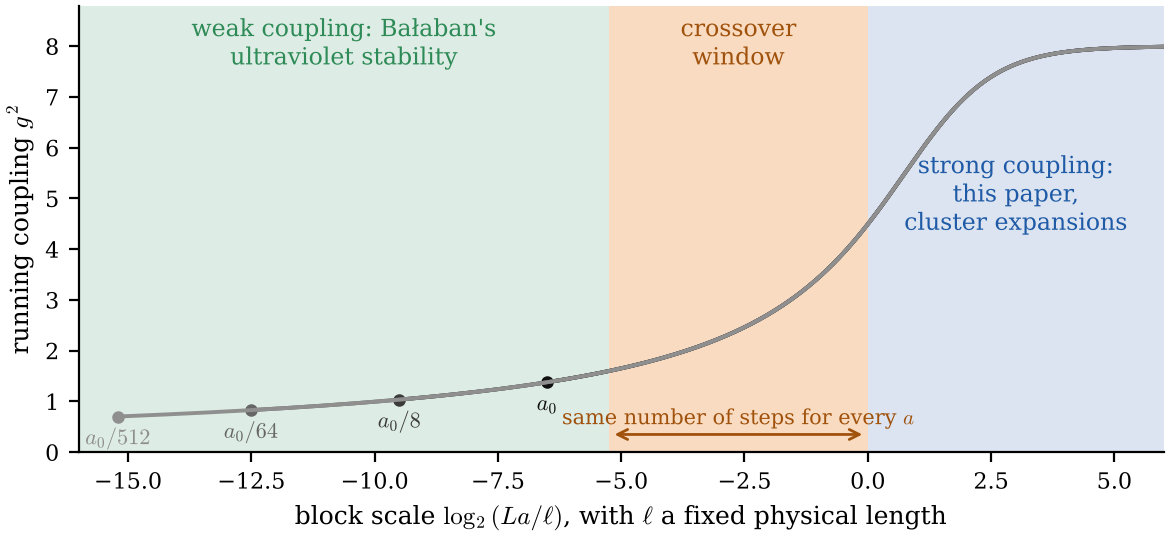
\includegraphics[width=0.96\textwidth]{figures/fig_scales.png}
\caption{The three regimes of the block-spin flow, with the running coupling
on the vertical axis and the block scale on the horizontal axis. The
strong-coupling end (left, blue) is controlled by the results of this paper
and by cluster expansions, the weak-coupling end (right, green) by
Ba{\l}aban's ultraviolet stability. No method controls the window between
them (orange), which every trajectory crosses in a number of steps
independent of the spacing. Trajectories started at the spacings
$a_0,a_0/8,a_0/64,a_0/512$ lie on one curve after the first steps, by
asymptotic freedom; the drawing is schematic, with the one-loop shape at weak
coupling.}
\label{fig:scales}
\end{figure*}

\begin{problem}[Crossover]\label{prob:crossover}
Show that at a block scale $a_*=c_*/\Lambda$ the effective density of the
four-dimensional $\SU(N)$ Wilson theory is a Wilson weight with coupling in
the regime of Theorem~B (or of a convergent cluster expansion) times
$\exp\sum_X\mathcal E_a(X)$, with $\mathcal E_a$ gauge invariant, local, and
small in the supremum norm over all block configurations, uniformly in the
spacing $a$ and in the volume.
\end{problem}

A solution of Problem~\ref{prob:crossover}, followed by the strong-coupling
analysis on the block lattice and reflection positivity of the fine theory,
would give a transfer-matrix gap of at least $ma$ at spacing $a$ with $m$
independent of $a$, which is the lattice form of the mass gap~\cite{BB26}; it
would also give a gap at every fixed coupling, by Proposition~\ref{prop:uniform}.
Problem~\ref{prob:crossover} is open.

\subsection{Where the available methods stop}

Each of the methods of this paper, and each of the routes proposed in the
literature, stops at a point that can be named.

\emph{Curvature.} Theorem~C shows that a lower bound on $\Ric-\Hess S$
uniform over configurations cannot exceed $\frac N2-4dN|\beta|$, because
the extremal fields of Theorem~A are allowed configurations. Any curvature
argument that goes further must exploit that those fields are rare, which
is an entropy statement, not a curvature statement.\footnote{Localisation
schemes and spectral conditions for Glauber dynamics~\cite{EKZ21,CE25}, and
the Polchinski-flow proof of log-Sobolev inequalities~\cite{BBo19}, replace
a uniform bound on the Hessian by a bound on the covariance of the measure
along a flow. For lattice gauge theory such a bound would itself require
control of correlations at the coupling in question, so these methods move
the difficulty rather than remove it. The classical relation between
log-Sobolev inequalities, spectral gaps and the decay of correlations is
in~\cite{Gro75,HS87,SZ92,Zeg96,MO94,OV00,Led01}.}

\emph{Single-link couplings.} Proposition~\ref{prop:ceiling} shows that no
single-link Wasserstein--Dobrushin argument goes beyond $\beta_W=2/9$, by
the configurations whose staples cancel. Couplings of larger blocks, as in
Theorem~G, avoid this ceiling, but then the finite computation has to be
done at the coupling in question.\footnote{For spin systems with compact
spin space Dobrushin's condition~\cite{Dob68,Dob70}, its Wasserstein form
and its consequences for decay and for transport and Poincar\'e
inequalities~\cite{Fol82,Kun82,Wu06,Oll09,DSa23} are classical, and the
Dobrushin--Shlosman finite-box conditions~\cite{DS85,DS87} are the block
version. Our gauge version, Definition~\ref{def:gds}, differs from the spin
version only through the identification of gauge-equivalent boundary data
and the interior gauge alignment of Lemma~\ref{lem:lift}.}

\emph{Finite-box criteria with corrections.} Feeding the renormalised action
of the crossover into Theorem~G requires, by Lemma~\ref{lem:stability}, a
smallness of the corrections $\mathcal E_a$ of order $\varepsilon/(|V|
|\partial V|)$. At order-one coupling the box that satisfies
$\mathrm{GDS}$ has to be large, and the required smallness shrinks with it,
so a solution of Problem~\ref{prob:crossover} has to produce corrections
that are small on the scale of the box, not only of the block.

\emph{Expansions in $1/N$ and the 't~Hooft regime.} The large-$N$ analyses of
lattice Yang--Mills theory~\cite{GW80,BG18,Nis25} and the string-trajectory
methods for Wilson loops~\cite{Cha16,Cha19,CPS25,CNS25a,CNS25b,AC25} control
the theory for $\beta$ below an $N$-independent threshold or for finite
gauge groups and Higgs models~\cite{Cao20,Cha20,FLV23}; they do not reach
order-one coupling at fixed $N$.

\emph{Abelian and two-dimensional models.} In four-dimensional $\U(1)$ theory
the weak-coupling phase is massless~\cite{Gut80,FS82}, and in three
dimensions Polyakov's mechanism gives confinement at all
couplings~\cite{Pol75a,FS81,GS23}. In two dimensions the $\SU(2)$ theory is
massive at every coupling (Proposition~\ref{prop:2d}). The closest analogue
of the four-dimensional crossover, the two-dimensional $\mathrm O(3)$ sigma
model at weak coupling, is asymptotically free and is believed to be massive
at every coupling~\cite{Pol75b}, but no proof of its mass gap at weak
coupling is published in refereed form.\footnote{The two-dimensional
$\mathrm O(N)$ models with $N\ge3$ share with four-dimensional Yang--Mills
theory a dimensionless coupling, asymptotic freedom and a dynamically
generated mass. For them as well the strong-coupling regime is controlled by
convergent expansions, the weak-coupling flow by perturbative renormalisation,
and the crossover between them is open. A proof for $\mathrm O(3)$ would be
the natural test of any method proposed for Problem~\ref{prob:crossover}.}
Three-dimensional $\SU(2)$ theory at large $\beta$ is open as well.

\emph{Order parameters.} The centre symmetry and the order parameters of
Fredenhagen and Marcu and of Bricmont and Fr\"ohlich~\cite{tH78,BF83,FM86,MP79}
distinguish
phases but give no estimate. Propositions~\ref{prop:centre}
and~\ref{prop:nolinear} identify the structural differences between $\SU(2)$
and $\U(1)$ that a proof would have to use; neither is an estimate, and
neither excludes a phase transition at intermediate coupling.

\section*{Data and code availability}

All proofs in this paper are by hand. The identities of
Lemma~\ref{lem:local} and Appendix~\ref{app:hessian}, the Barta and Riccati
computations of Appendix~\ref{app:vmf}, the extremal values in Theorem~A and
the numerical values quoted after Conjecture~\ref{conj:quarter} and
Proposition~\ref{prop:reduction} were also checked independently, in exact
arithmetic where possible, and the bound of Theorem~A against the
numerically computed Hessian on random configurations; these checks are
archived with the source of this paper in the repository
\texttt{creelie/4Y-M}. Deep Bhattacharjee carried out the computations and
checks in Python (SymPy, NumPy, SciPy) with AI assistance from Claude
(Anthropic); both authors approved the final text.

\section*{Ethical declarations}

\emph{Funding.} None. \emph{Competing interests.} None.

\appendix

\section{The Hessian of a plaquette}\label{app:hessian}

\subsection{The perturbed plaquette}

Perturb every link variable along its geodesic, $Q_e(t)=e^{tX_e}Q_e$. The
plaquette variable becomes
\[
Q_p(t)=e^{tX_{e_1}}Q_{e_1}\,e^{tX_{e_2}}Q_{e_2}\,Q_{e_3}^*e^{-tX_{e_3}}\,
Q_{e_4}^*e^{-tX_{e_4}} .
\]
Move each exponential to the base point. Since $Q_{e_1}e^{tX}=
e^{tQ_{e_1}XQ_{e_1}^*}Q_{e_1}$ and $Q_{e_3}^*e^{-tX_{e_3}}Q_{e_4}^*=
Q_{e_3}^*Q_{e_4}^*\,e^{-tQ_{e_4}X_{e_3}Q_{e_4}^*}$, the transported vectors
of~\eqref{eq:transport} give
\[
Q_p(t)=a(t)\,W\,b(t),\qquad a(t)=e^{tY_1}e^{tY_2},\quad b(t)=e^{-tY_3}
e^{-tY_4},
\]
with $W=Q_p$. Now $a(0)=b(0)=1$, $a'(0)=Y_1+Y_2$, $b'(0)=-(Y_3+Y_4)$,
$a''(0)=Y_1^2+2Y_1Y_2+Y_2^2$ and $b''(0)=Y_3^2+2Y_3Y_4+Y_4^2$, so
\[
\frac{d^2}{dt^2}Q_p(t)\Big|_{t=0}=a''(0)W+2a'(0)Wb'(0)+Wb''(0).
\]
Taking $\ReTr$ and using the cyclicity of the trace,
$\ReTr(WY_i^2)=\ReTr(Y_i^2W)$ and $\ReTr(WY_3Y_4)=\ReTr(Y_3Y_4W)$, gives
\eqref{eq:fp}.

\subsection{The corner terms}

Fix the plaquette $p$ with base point $x$ in the plane $\mu<\nu$. Its four
corners are the vertices $x$, $x+\hat\mu$, $x+\hat\nu$, $x+\hat\mu+\hat\nu$,
and at each corner two of its links meet, one of direction $\mu$ and one of
direction $\nu$. In $|D_yX|^2$ the end of a link at $y$ enters with the sign
$+$ if the link leaves $y$ and with the sign $-$ if it arrives at $y$, an
arriving link $(y-\hat\lambda,\lambda)$ being transported by
$Q_{y-\hat\lambda,\lambda}^*\,\cdot\,Q_{y-\hat\lambda,\lambda}$. The cross term
of the two ends at each corner is:
\begin{itemize}[leftmargin=*]
\item at $x$, $e_1$ and $e_4$ both leave: $2\ip{X_{e_1}}{X_{e_4}}=2\ip{Y_1}
{Y_4}$;
\item at $x+\hat\mu$, $e_1$ arrives and $e_2$ leaves:
$-2\ip{X_{e_2}}{Q_{e_1}^*X_{e_1}Q_{e_1}}=-2\ip{Y_2}{Y_1}$, by invariance of
the inner product under conjugation;
\item at $x+\hat\nu$, $e_4$ arrives and $e_3$ leaves:
$-2\ip{X_{e_3}}{Q_{e_4}^*X_{e_4}Q_{e_4}}=-2\ip{Y_3}{Y_4}$;
\item at $x+\hat\mu+\hat\nu$, $e_2$ and $e_3$ both arrive:
$2\ip{Q_{e_2}^*X_{e_2}Q_{e_2}}{Q_{e_3}^*X_{e_3}Q_{e_3}}$. Since
$X_{e_2}=Q_{e_1}^*Y_2Q_{e_1}$ and $X_{e_3}=Q_{e_4}^*Y_3Q_{e_4}$, this
equals $2\ip{Y_2}{WY_3W^*}$.
\end{itemize}
The sum is the corner form~\eqref{eq:corner}. Conversely every cross term of
$\sum_y|D_yX|^2$ between ends of two perpendicular directions $\mu\ne\nu$ at a
vertex $y$ is one of these: the two ends determine a quadrant of the plane
$\mu\nu$ at $y$, hence a unique plaquette with a corner at $y$.

\subsection{The diagonal blocks}

Assume $W=D=\operatorname{diag}(w_1,\dots,w_N)$, as in the proof of
Lemma~\ref{lem:local}, and expand every trace in matrix entries:
\[
\begin{aligned}
\ReTr(Y_iY_jW)&=\operatorname{Re}\sum_{a,b}(Y_i)_{ab}(Y_j)_{ba}w_a,\\
\ReTr(Y_iWY_j)&=\operatorname{Re}\sum_{a,b}(Y_i)_{ab}w_b(Y_j)_{ba}.
\end{aligned}
\]
The terms with $a=b$ involve only the diagonal entries $(Y_i)_{aa}=\mathrm
iy_i$, $y_i\in\R$. With $w_a=e^{\mathrm i\varphi}$ they contribute
$-y_iy_j\cos\varphi$ to both traces, so the diagonal part of $f_p$ is
\[
\begin{aligned}
-\cos\varphi\Bigl[\sum_iy_i^2+2y_1y_2+2y_3y_4&-2(y_1+y_2)(y_3+y_4)\Bigr]\\
&=-\cos\varphi\,s^2,
\end{aligned}
\]
with $s=y_1+y_2-y_3-y_4$. The inner products $\ip{Y_i}{Y_j}$ and
$\ip{Y_2}{WY_3W^*}$ contribute $y_iy_j$ and $y_2y_3$ (the phases cancel), so
the diagonal part of $c_p$ is $2y_1y_4-2y_1y_2+2y_2y_3-2y_3y_4$. Expanding the
squares,
\[
\begin{aligned}
(y_1+y_3)^2&+(y_2+y_4)^2+s^2\\
&=2\sum_iy_i^2-\bigl(2y_1y_4-2y_1y_2+2y_2y_3-2y_3y_4\bigr),
\end{aligned}
\]
and therefore the diagonal block of $F=2\sum|Y_i|^2-f_p-c_p$ is
$(y_1+y_3)^2+(y_2+y_4)^2+(1+\cos\varphi)s^2$.

\subsection{The pair blocks}

Fix $a\ne b$ and put $z_i=(Y_i)_{ab}$, so that $(Y_i)_{ba}=-\bar z_i$. The
terms of the traces at the positions $(a,b)$ and $(b,a)$ give
\begin{align*}
\ReTr(Y_iY_jW)&\to-\operatorname{Re}(z_i\bar z_jw_a+\bar z_iz_jw_b),\\
\ReTr(Y_iWY_j)&\to-\operatorname{Re}(z_i\bar z_jw_b+\bar z_iz_jw_a),\\
\ip{Y_i}{Y_j}&\to2\operatorname{Re}(\bar z_iz_j),\\
\ip{Y_2}{WY_3W^*}&\to2\operatorname{Re}(\bar z_2z_3w_a\bar w_b),
\end{align*}
and $|Y_i|^2$ contains $2|z_i|^2$. Write $w_a=e^{\mathrm i(\chi+\theta)}$,
$w_b=e^{\mathrm i(\chi-\theta)}$ and $m=\cos\chi$. Collecting terms, the pair
block of $F$ is $z^*M(m,\theta)z$ for the Hermitian matrix with diagonal
entries $4+2m\cos\theta$ and upper off-diagonal entries
\begin{align*}
M_{12}&=M_{34}=2+2me^{-\mathrm i\theta},&
M_{13}&=M_{24}=-2me^{\mathrm i\theta},\\
M_{14}&=-2-2me^{\mathrm i\theta},&
M_{23}&=-2e^{2\mathrm i\theta}-2me^{\mathrm i\theta}.
\end{align*}
Only $m=\cos\chi$ appears, not $\sin\chi$: in each term the two phases enter
through $w_a+w_b=2e^{\mathrm i\chi}\cos\theta$ or through the real parts of
the combinations displayed.\footnote{One way to see that $\sin\chi$ drops
out is to note that replacing $W$ by $\bar W$ and every $Y_i$ by $\bar Y_i$
leaves $F$ unchanged, since all the terms are real parts of traces, and maps
$\chi\mapsto-\chi$, $\theta\mapsto-\theta$ together with $z\mapsto\bar z$.
The explicit collection of terms confirms that the coefficients depend on
$\chi$ only through $\cos\chi$.} The matrix is affine in $m$, and the
substitution $\theta\mapsto\theta+\pi$ changes $e^{\mathrm i\theta}$ and
$\cos\theta$ into their negatives while leaving $e^{2\mathrm i\theta}$
unchanged, so $M(-1,\theta)=M(1,\theta+\pi)$. Since $m\in[-1,1]$,
\[
M(m,\theta)=\frac{1+m}2M(1,\theta)+\frac{1-m}2M(1,\theta+\pi),
\]
and it suffices to show $M(1,\theta)\ge0$ for every $\theta$.

Let $\Delta=\operatorname{diag}(1,e^{\mathrm i\theta/2},e^{-\mathrm i\theta},
e^{-\mathrm i\theta/2})$ and $c=\cos(\theta/2)$. A direct multiplication gives
the real symmetric matrix
\[
\Delta^*M(1,\theta)\Delta=\begin{pmatrix}2+4c^2&4c&-2&-4c\\4c&2+4c^2&-4c&-2\\
-2&-4c&2+4c^2&4c\\-4c&-2&4c&2+4c^2\end{pmatrix},
\]
using $4+2\cos\theta=2+4c^2$ and $2+2e^{-\mathrm i\theta}=4ce^{-\mathrm i
\theta/2}$. Its quadratic form in $u\in\C^4$ is
\begin{multline*}
2c^2\bigl(|u_1+u_3|^2+|u_2+u_4|^2\bigr)+(1+c)^2|u_1+u_2-u_3-u_4|^2\\
+(1-c)^2|u_1-u_2-u_3+u_4|^2,
\end{multline*}
as one checks by comparing coefficients: the diagonal coefficient is
$2c^2+(1+c)^2+(1-c)^2=2+4c^2$, the coefficient of $\operatorname{Re}(\bar
u_1u_2)$ is $2\bigl[(1+c)^2-(1-c)^2\bigr]=8c$, that of $\operatorname{Re}(\bar
u_1u_3)$ is $2\bigl[2c^2-(1+c)^2-(1-c)^2\bigr]=-4$, that of
$\operatorname{Re}(\bar u_1u_4)$ is $2\bigl[-(1+c)^2+(1-c)^2\bigr]=-8c$, and the
others follow by the symmetry $(u_1,u_2,u_3,u_4)\mapsto(u_3,u_4,u_1,u_2)$
with a sign. Every pair block is therefore positive semidefinite.

\section{The single-link law of SU(2)}\label{app:vmf}

\subsection{Barta's inequality}

Let $\rho(\theta)=\sin^2\theta\,e^{\kappa\cos\theta}$ on $(0,\pi)$, let $V$
be a continuous potential, and let
\[
T=-\rho^{-1}\partial_\theta\,\rho\,\partial_\theta+V .
\] If $\psi>0$ is smooth on $(0,\pi)$ with
$\rho\psi^2=O(\sin^4\theta)$ at the end points and $T\psi\ge\lambda_0\psi$,
then
\[
\int(|h'|^2+Vh^2)\rho\,d\theta\ge\lambda_0\int h^2\rho\,d\theta
\]
for every smooth $h$ vanishing to first order at $0$ and $\pi$. Indeed, writing
$h=\psi u$ and integrating by parts, the boundary terms $\rho\psi\psi'u^2$
vanish and
\[
\int(|h'|^2+Vh^2)\rho=\int\rho\psi^2|u'|^2+\int\frac{T\psi}\psi\,h^2\rho
\ \ge\ \lambda_0\int h^2\rho .
\]
This is the inequality of Barta~\cite{Bar37} in the form of a ground state
transformation.

\subsection{The computations of Lemma~\ref{lem:vmf}}

The generator of the reversible diffusion of $\nu_b$ on $S^3$ is
$L=\Delta_{S^3}+\kappa\nabla x_1\cdot\nabla$. In the polar angle $\theta$
from $e_1$ the round metric is $d\theta^2+\sin^2\theta\,g_{S^2}$, so
$\Delta_{S^3}=\partial_\theta^2+2\cot\theta\,\partial_\theta+\sin^{-2}\theta\,
\Delta_{S^2}$, and $\nabla x_1\cdot\nabla=-\sin\theta\,\partial_\theta$. On
$h(\theta)Y_\ell$ with a spherical harmonic $Y_\ell$ of degree $\ell$ on $S^2$
the operator acts as $L_\ell=\partial_\theta^2+b\,\partial_\theta-\ell(\ell+1)
\sin^{-2}\theta$, $b=2\cot\theta-\kappa\sin\theta=\rho'/\rho$, so
$-L_\ell=T$ with $V=\ell(\ell+1)\sin^{-2}\theta$.

\emph{Degree $\ell\ge1$.} Take $\psi=\sin\theta\,e^{a\kappa\cos\theta}$. Then
$\psi'/\psi=\cot\theta-a\kappa\sin\theta$ and
$\psi''/\psi=(\psi'/\psi)^2+(\psi'/\psi)'$, and a short computation gives
\[
\frac{-L_1\psi}\psi=3+(1+5a)\kappa\cos\theta-a(1+a)\kappa^2\sin^2\theta .
\]
For $a=-\frac15$ this is $3+\frac4{25}\kappa^2\sin^2\theta\ge3$. Since
$V=\ell(\ell+1)\sin^{-2}\theta\ge2\sin^{-2}\theta$ for $\ell\ge1$, Barta's
inequality gives $-L_\ell\ge3$ on every sector with $\ell\ge1$.

\emph{Degree $\ell=0$.} Let $g(\theta)$ be a zonal eigenfunction,
$-L_0g=\lambda g$, $g$ not constant, so that $g'(0)=g'(\pi)=0$. Differentiating
$g''+bg'=-\lambda g$ gives, for $h=g'$,
\[
-\bigl(h''+bh'\bigr)-b'h=\lambda h,\qquad -b'=\frac2{\sin^2\theta}+\kappa
\cos\theta,
\]
so $h$ is an eigenfunction of $T$ with $V=2\sin^{-2}\theta+\kappa\cos\theta$,
with eigenvalue $\lambda$, and $h\not\equiv0$ vanishes at both ends. With the
same $\psi$,
\[
\frac{T\psi}\psi=3+(2+5a)\kappa\cos\theta-a(1+a)\kappa^2\sin^2\theta,
\]
which for $a=-\frac25$ is $3+\frac6{25}\kappa^2\sin^2\theta\ge3$. Barta's
inequality applied to $h$ gives $\lambda\ge3$. Together with the case
$\ell\ge1$ every nonzero eigenvalue of $-L$ is at least $3$, which is
Lemma~\ref{lem:vmf}; the spectrum is discrete because $S^3$ is compact and
the drift is smooth.

\subsection{Moments}

The density of $t=x_1$ under $\nu_b$ is proportional to $(1-t^2)^{1/2}e^{
\kappa t}$. For every smooth $\phi$ on $[-1,1]$,
\[
\frac d{dt}\Bigl[(1-t^2)^{3/2}e^{\kappa t}\Bigr]=(1-t^2)^{1/2}e^{\kappa t}
\bigl(\kappa(1-t^2)-3t\bigr),
\]
and integration by parts gives $\E[\phi'(t)(1-t^2)]=\E\bigl[\phi(t)\bigl(3t-
\kappa(1-t^2)\bigr)\bigr]$. With $\phi=1$ this is $\kappa\E(1-x_1^2)=3\E x_1$,
the identity of Lemma~\ref{lem:moments}(i). With $\phi=t^k$ it gives the
recursion
\[
m_{k+2}=m_k-\frac{k+3}\kappa\,m_{k+1}+\frac k\kappa\,m_{k-1},\qquad m_k=\E
x_1^k,
\]
from $m_0=1$ and $m_1=A$; all polynomial moments of $\nu_b$ are rational in
$\kappa$ and $A(\kappa)$.\footnote{For instance $m_2=1-3A/\kappa$,
$m_3=A-3/\kappa+12A/\kappa^2$ and $m_4=m_2-5m_3/\kappa+2A/\kappa$. The joint moments
with $x_2,x_3,x_4$ follow from exchangeability:
$\E[\phi(x_1)x_2^2]=\frac13\E[\phi(x_1)(1-x_1^2)]$.}

\subsection{The Riccati barriers}

By Lemma~\ref{lem:moments}(i), $A$ solves $A'=\mathcal F(\kappa,A):=1-A^2-
3A/\kappa$ on $(0,\infty)$, and $A(\kappa)=\frac\kappa4-\frac{\kappa^3}{96}+
O(\kappa^5)$ from the series of $I_1$ and $I_2$. Let $s=\sqrt{\kappa^2+4}$,
$u=\sqrt{\kappa^2+9}$, $\phi_-=\kappa/(2+s)$ and $\phi_+=\kappa/(1+u)$. Direct
differentiation gives
\[
\begin{aligned}
\phi_-'-\mathcal F(\kappa,\phi_-)&=-\frac{\kappa^2}{s(s+2)^2}\le0,\\
\phi_+'-\mathcal F(\kappa,\phi_+)&=\frac{(u-3)^2}{u(1+u)^2}\ge0,
\end{aligned}
\]
and $\phi_\pm=\frac\kappa4+O(\kappa^3)$.\footnote{For the first identity write
$\phi_-=(s-2)/\kappa$, which follows from $s^2-4=\kappa^2$; then
$\phi_-'=(\kappa^2/s-s+2)/\kappa^2$ and $1-\phi_-^2-3\phi_-/\kappa=
(\kappa^2-(s-2)^2-3(s-2))/\kappa^2$, and the difference simplifies with
$s^2=\kappa^2+4$. The second is the same computation with
$\phi_+=\kappa(u-1)/(u^2-1)=\kappa(u-1)/(\kappa^2+8)$ in place of $\phi_-$
and $u^2=\kappa^2+9$ in place of $s^2=\kappa^2+4$. After clearing the denominator $\kappa^2(1+u)^2$ the
numerator becomes $\kappa^2(u-3)^2/u$, which is the stated residual.} The comparison is singular at $0$
because of the term $3A/\kappa$, and we carry it out with an integrating
factor. Let $D=A-\phi_-$. Then
\[
\begin{aligned}
D'&=\mathcal F(\kappa,A)-\mathcal F(\kappa,\phi_-)-\bigl(\phi_-'-\mathcal F(
\kappa,\phi_-)\bigr)\\
&=-\Bigl(A+\phi_-+\frac3\kappa\Bigr)D+R,
\end{aligned}
\]
with $R=\kappa^2/(s(s+2)^2)\ge0$. Put $\mu(\kappa)=\kappa^3\exp\int_0^\kappa
(A+\phi_-)$. Then $(\mu D)'=\mu R\ge0$, and $\mu D=O(\kappa^6)\to0$ as
$\kappa\to0$, so $\mu D\ge0$ and $A\ge\phi_-$. The same argument with
$D=\phi_+-A$ and $R=(u-3)^2/(u(1+u)^2)$ gives $A\le\phi_+$. This is
Lemma~\ref{lem:moments}(ii).

\section{The weighted coupling}\label{app:weighted}

We prove Lemma~\ref{lem:weighted}. Let $Q,Q'$ be two fields such that for
every link $Q'_e$ is not in the cut locus of $Q_e$, which is the situation
in~\eqref{eq:rhoe}, and let $\gamma_e\colon[0,1]\to G$ be the minimal geodesic
from $Q_e$ to $Q'_e$, of constant speed $\rho_e$. The product
$\gamma(\tau)=(\gamma_e(\tau))_e$ is a geodesic of the product manifold, with
velocity $V(\tau)=(\dot\gamma_e(\tau))_e$ and $|V_e|=\rho_e$.

\emph{Step 1: an integral identity.} Let $V^{(e)}$ be the vector field along
$\gamma$ that equals $\dot\gamma_e$ at the link $e$ and vanishes elsewhere.
It is parallel along $\gamma$, because each $\dot\gamma_e$ is parallel along
the geodesic $\gamma_e$ and the Levi-Civita connection of a product is the
product connection. Hence
\[
\frac d{d\tau}\ip{\nabla S(\gamma(\tau))}{V^{(e)}(\tau)}=\Hess S\bigl(V(\tau),
V^{(e)}(\tau)\bigr),
\]
and integrating from $0$ to $1$, with $\ip{\nabla S}{V^{(e)}}=\rho_e\ip{\nabla
S}{\dot\gamma_e/\rho_e}$,
\begin{equation}\label{eq:keyid}
\rho_e\bigl(\ip{\nabla S}{\hat\gamma_e}(Q')-\ip{\nabla S}{\hat\gamma_e}(Q)
\bigr)=\int_0^1\Hess S\bigl(V,V^{(e)}\bigr)\,d\tau,
\end{equation}
where $\hat\gamma_e=\dot\gamma_e/\rho_e$ is the unit tangent written
$\dot\gamma_e$ in~\eqref{eq:rhoe}.

\emph{Step 2: symmetrisation.} Multiply~\eqref{eq:keyid} by $w_e$ and sum over
$e$. The sum converges absolutely, because $\rho_e\le\pi\sqrt2$ is bounded,
$\sum_ew_e<\infty$, and the Hessian is a sum of finite-range blocks. Write
$H_{ef}$ for the block of $\Hess S$ between the links $e$ and $f$. Then
\[
\begin{aligned}
\sum_ew_e\Hess S(V,V^{(e)})&=\sum_{e,f}w_fH_{ef}(V_e,V_f)\\
&=\sum_{e,f}\frac{w_e+w_f}2H_{ef}(V_e,V_f),
\end{aligned}
\]
the second equality by the symmetry $H_{ef}(V_e,V_f)=H_{fe}(V_f,V_e)$. Put
$Y_e=w_e^{1/2}V_e$, so that $|Y|^2=\sum_ew_e\rho_e^2<\infty$. With
$r=w_e/w_f$,
\[
\frac{w_e+w_f}{2\sqrt{w_ew_f}}=\frac{r^{1/2}+r^{-1/2}}2=1+\frac12\bigl(r^{1/4}
-r^{-1/4}\bigr)^2,
\]
and therefore
\[
\sum_ew_e\Hess S(V,V^{(e)})=\Hess S(Y,Y)+B,
\]
with $B=\sum_{e\ne f}H_{ef}(Y_e,Y_f)\cdot\frac12(r^{1/4}-r^{-1/4})^2$, the
diagonal terms $e=f$ having $r=1$.

\emph{Step 3: the two estimates.} Theorem~A applies to the square-summable
vector $Y$ and gives $|\Hess S(Y,Y)|=N|\beta||\Hess S_0(Y,Y)|\le4dN|\beta|
|Y|^2$. In $B$ only links $e\ne f$ in a common plaquette contribute, and two
distinct links lie in at most one common plaquette. Their mixed term in
$f_p$ is one of $2\ReTr(Y_iY_jW)$, $-2\ReTr(Y_iWY_j)$, and since
$|\Tr(XYW)|\le|X||Y|$ for unitary $W$, the bilinear form satisfies
$|H_{ef}(Y_e,Y_f)|\le N|\beta||Y_e||Y_f|$ for each of the two orders. The
end points of such links have graph distances to the origin that differ by at
most one, so $r\in[a^{-1},a]$ and $\frac12(r^{1/4}-r^{-1/4})^2\le(\sqrt a-1)^2/
(2\sqrt a)$. Every link has $6(d-1)$ neighbours in common plaquettes, so
\[
\begin{aligned}
|B|&\le N|\beta|\frac{(\sqrt a-1)^2}{2\sqrt a}\sum_{e\ne f}|Y_e||Y_f|\\
&\le3(d-1)N|\beta|\frac{(\sqrt a-1)^2}{\sqrt a}|Y|^2,
\end{aligned}
\]
by $|Y_e||Y_f|\le\frac12(|Y_e|^2+|Y_f|^2)$. Integrating over $\tau$, and using
that $|Y|^2=\sum_ew_e\rho_e^2$ does not depend on $\tau$, gives
\[
\sum_ew_e\rho_e\bigl(\ip{\nabla S}{\hat\gamma_e}(Q')-\ip{\nabla S}{\hat
\gamma_e}(Q)\bigr)\le\bigl(C_{\rm Ric}-K_a\bigr)\sum_ew_e\rho_e^2,
\]
which is Lemma~\ref{lem:weighted}. The constant of Shen, Zhu and
Zhu~\cite[Sec.~5]{SZZ23} arises if the weighted sum is estimated link by link
with~\eqref{eq:szzbound}; the gain comes from estimating the whole quadratic
form $\Hess S(Y,Y)$ with Theorem~A and paying only for the commutator of the
weights.

\section{A Kantorovich--Dobrushin comparison}\label{app:dobrushin}

Let $\Omega=(S^3)^E$ with the chordal metric $\delta$ on each factor, of
diameter $2$, and let $\gamma_e(\cdot\mid\omega)$ be the single-link
conditional laws of the $\SU(2)$ Wilson theory. Let $C_{ee'}$ be the
coefficients of the proof of Theorem~E, $\alpha<1$ their maximal row and
column sum, and $|e-e'|$ the Euclidean distance of link midpoints; links in a
common plaquette have $|e-e'|\le1$. Fix $\lambda>0$ with $\theta:=\alpha e^
\lambda<1$.

\begin{lemma}\label{lem:comparison}
Let $S\subset E$ be finite, possibly empty, and let $\mu_1,\mu_2$ be
probability measures on $\Omega$ that are invariant under the resampling
$\gamma_e$ of every link $e\notin S$. Let $T\subset E\setminus S$ be finite
and $w_b=e^{-\lambda\dist(b,T)}$. There is a coupling $\pi$ of $\mu_1,\mu_2$
such that $\varrho(b)=\E_\pi\delta(\sigma_b,\sigma'_b)$ satisfies
\[
\sum_{b\notin S}w_b\varrho(b)\le\frac{2\theta}{1-\theta}\sum_{z\in S}w_z .
\]
In particular $\sum_{b\in T}\varrho(b)\le\frac{2\theta}{1-\theta}|S|\,e^{-
\lambda\dist(S,T)}$, and if $S=\emptyset$ then $\mu_1=\mu_2$.
\end{lemma}

\begin{proof}
\emph{A minimal coupling.} The set of couplings of $\mu_1$ and $\mu_2$ is
weakly compact, and $\Psi(\pi)=\sum_bw_b\E_\pi\delta(\sigma_b,\sigma'_b)$ is
weakly continuous, since $\delta$ is continuous and bounded and $\sum_bw_b<
\infty$. Let $\pi^*$ be a minimiser and $\varrho$ its link distances.

\emph{Resampling one link.} Fix $e\notin S$. By~\cite[Cor.~5.22]{Vil09}
there is a measurable map assigning to each pair $(\omega,\omega')$ an
optimal coupling of $\gamma_e(\cdot\mid\omega)$ and $\gamma_e(\cdot\mid
\omega')$ for $\delta$. Sample $(\sigma,\sigma')\sim\pi^*$ and replace the pair
$(\sigma_e,\sigma'_e)$ by a sample of that coupling; since both $\mu_i$ are
$\gamma_e$-invariant, the result is again a coupling of $\mu_1,\mu_2$, and only
the link $e$ changes. Changing the finitely many links that enter
$\gamma_e$ one at a time and using the triangle inequality for $W_1$,
\[
W_1\bigl(\gamma_e(\cdot\mid\sigma),\gamma_e(\cdot\mid\sigma')\bigr)\le
\sum_{e'}C_{ee'}\delta(\sigma_{e'},\sigma'_{e'}).
\]
Minimality of $\pi^*$ therefore gives $\varrho(e)\le\sum_{e'}C_{ee'}
\varrho(e')$ for every $e\notin S$.

\emph{Summation.} Multiply by $w_e$ and sum over $e\notin S$. Where
$C_{ee'}\ne0$ the links are in a common plaquette, so $\dist(e,T)\ge\dist(e',
T)-1$ and $w_e\le e^\lambda w_{e'}$. With the column sums bounded by
$\alpha$,
\[
\begin{aligned}
\sum_{e\notin S}w_e\varrho(e)&\le e^\lambda\sum_{e'}w_{e'}\varrho(e')\sum_eC_{ee'}\\
&\le\theta\Bigl[\sum_{e'\notin S}w_{e'}\varrho(e')+\sum_{z\in S}w_z\varrho(z)
\Bigr].
\end{aligned}
\]
All sums are finite, and $\varrho(z)\le2$ on $S$; rearranging gives the first
claim. On $T$ the weights equal $1$, and $w_z\le e^{-\lambda\dist(S,T)}$ for
$z\in S$. If $S=\emptyset$ then $\varrho\equiv0$, so $\pi^*$ is supported on the
diagonal and $\mu_1=\mu_2$.
\end{proof}

\begin{corollary}\label{cor:decay}
In the range of Theorem~E there is exactly one Gibbs measure $\mu$, and for
a local function $F$ with support $S_F$ that is $L_F$-Lipschitz in each
link variable, and a bounded measurable $H$ with finite support $S_H$
disjoint from $S_F$,
\[
|\Cov_\mu(F,H)|\le\|H\|_\infty L_F\,\frac{2\theta}{1-\theta}\,|S_H|\,
e^{-\lambda\dist(S_F,S_H)} .
\]
\end{corollary}

\begin{proof}
Gibbs measures are invariant under every $\gamma_e$, so the case
$S=\emptyset$ of Lemma~\ref{lem:comparison} gives uniqueness, and Gibbs
measures exist by compactness. Let $\mu^u=\mu(\cdot\mid\sigma_{S_H}=u)$ be a
regular conditional probability~\cite[Ch.~3]{Kal21}; for $\mu$-almost every
$u$ it is invariant under $\gamma_e$ for every $e\notin S_H$, because the
conditional law of $\sigma_e$ given everything else is $\gamma_e$ and does not
depend on how $\sigma_{S_H}$ was fixed. Writing
$\Cov_\mu(F,H)=\int H(u)\bigl[\mu^u(F)-\int\mu^{u'}(F)\mu(du')\bigr]\mu(du)$,
\[
|\Cov_\mu(F,H)|\le\|H\|_\infty\operatorname*{ess\,sup}_{u,u'}|\mu^u(F)-
\mu^{u'}(F)| .
\]
Apply Lemma~\ref{lem:comparison} to $\mu^u,\mu^{u'}$ with $S=S_H$ and
$T=S_F$: $|\mu^u(F)-\mu^{u'}(F)|\le L_F\sum_{b\in S_F}\varrho(b)$, and the
second claim of the lemma completes the proof.
\end{proof}

The decay of Theorem~E is Corollary~\ref{cor:decay}; the rate $\lambda$ can
be any number below $-\log\alpha$.

\section{Two-dimensional estimates}\label{app:twod}

\subsection{Total variation under a bounded change of density}

\begin{lemma}\label{lem:tanh}
Let $P,P'$ be probability measures with $dP'/dP=e^\phi/\E_Pe^\phi$, where
$\phi$ has oscillation at most $s$. Then $\|P-P'\|_{\rm TV}\le\tanh(s/4)$, and
the bound is attained.
\end{lemma}

\begin{proof}
We may assume $0\le\phi\le s$. For an event $A$ with $P(A)=x$ put
$p=\E_P[e^\phi;A]\in[x,e^sx]$ and $q=\E_P[e^\phi;A^c]\in[1-x,e^s(1-x)]$.
Then $P'(A)=p/(p+q)$ increases in $p$ and decreases in $q$, so
\[
P'(A)-P(A)\le\frac{e^sx}{e^sx+1-x}-x=:g(x).
\]
The derivative $g'(x)=e^s/(1+x(e^s-1))^2-1$ vanishes at $1+x(e^s-1)=
e^{s/2}$, that is $x=1/(e^{s/2}+1)$, where $g=x(e^{s/2}-1)=\tanh(s/4)$. The
value is attained for $\phi=s\mathbf 1_A$ with this $P(A)$.
\end{proof}

If $P_i$ has density proportional to $\varrho g_i$ with $g_i\in[1-\epsilon,1+
\epsilon]$, then $\log(g_1/g_2)$ has oscillation at most $2\log\frac{1+\epsilon}
{1-\epsilon}$, and Lemma~\ref{lem:tanh} gives $\|P_1-P_2\|_{\rm TV}\le
\epsilon$. The weaker bound $2\epsilon/(1-\epsilon^2)$ used in the proof of
Proposition~\ref{prop:2d} follows directly: with $c_i=\int\varrho g_i\in
[(1-\epsilon)c,(1+\epsilon)c]$, $c=\int\varrho$, one has
$|g_1/c_1-g_2/c_2|\le\frac1c\bigl(\frac{1+\epsilon}{1-\epsilon}-\frac{1-
\epsilon}{1+\epsilon}\bigr)=\frac{4\epsilon}{c(1-\epsilon^2)}$, and the total
variation is half the $L^1$ norm.

\subsection{The character expansion}

On $\SU(2)$ write $U$ with eigenvalues $e^{\pm\mathrm i\vartheta}$, so that
$\Tr U=2\cos\vartheta$, the Haar measure of class functions is
$\frac2\pi\sin^2\vartheta\,d\vartheta$, and the character of spin $j$ is
$\chi_j=\sin((2j+1)\vartheta)/\sin\vartheta$. The coefficient of $\chi_j$ in
$w(U)=e^{\beta\cos\vartheta}$ is
\[
\begin{aligned}
\frac2\pi\int_0^\pi e^{\beta\cos\vartheta}&\sin((2j+1)\vartheta)\sin\vartheta
\,d\vartheta\\
&=I_{2j}(\beta)-I_{2j+2}(\beta)=\frac{2(2j+1)}\beta I_{2j+1}(\beta),
\end{aligned}
\]
by $2\sin A\sin B=\cos(A-B)-\cos(A+B)$, the integral $\frac1\pi\int_0^\pi
e^{\beta\cos\vartheta}\cos(n\vartheta)d\vartheta=I_n(\beta)$ and the recurrence
$I_{n-1}-I_{n+1}=\frac{2n}xI_n$~\cite[Sec.~3.71]{Wat44}. So
$c_0=\int w=2I_1(\beta)/\beta$ and $f=w/c_0=\sum_j(2j+1)a_j\chi_j$ with
$a_j=I_{2j+1}(\beta)/I_1(\beta)\in(0,1)$ for $j\ge\frac12$, since $I_n(\beta)$
decreases in $n$ for $\beta>0$. Schur orthogonality gives $\chi_j*\chi_k=
\delta_{jk}\chi_j/(2j+1)$, hence $f^{*m}=\sum_j(2j+1)a_j^m\chi_j$. Since
$|\chi_j|\le2j+1$ with equality at $U=1$,
\[
\begin{aligned}
\varepsilon_m=\sup_U|f^{*m}(U)-1|&=\sum_{j\ge1/2}(2j+1)^2a_j^m\\
&\le a_{1/2}^{m-1}\sum_{j\ge1/2}(2j+1)^2a_j,
\end{aligned}
\]
which is finite because $I_n(\beta)\le(\beta/2)^ne^{\beta}/n!$, and tends to
zero geometrically in $m$.

\subsection{Disk integration}

\begin{proof}[Proof of Lemma~\ref{lem:disk}]
We use the lemma only for rectangles, and prove it for them. Order the
plaquettes of the rectangle $D$ row by row, from left to right, and let
$D_i$ be the union of the first $i$. Each $D_i$ is a staircase, hence a
topological disk, and $p_{i+1}$ meets $D_i$ along a path $\gamma$ of one or
two consecutive links (its left side, its lower side, or both, which meet at
a corner). We show by induction that integrating $\prod_{p\subset D_i}w(U_p)$
over the interior links of $D_i$ gives $c_0^if^{*i}(\mathrm{hol}_{\partial
D_i})$; $f$ is a class function, so the base point of the holonomy does not
matter. For $i=1$ there is nothing to integrate. In the step, write
$\partial D_i=\gamma\cdot\beta$ and $\partial p_{i+1}=\gamma^{-1}\cdot\eta$,
with holonomies $\Gamma B$ and $\Gamma^{-1}H$, where $\Gamma$ is the product of
the link variables of $\gamma$. The new interior links are those of $\gamma$,
and the integrand depends on them only through $\Gamma$. If $\gamma$ has two
links, $\Gamma=U_{e_1}U_{e_2}$ is Haar distributed for each fixed $U_{e_1}$.
In both cases the integral over the links of $\gamma$ is
\[
c_0^{i+1}\int f^{*i}(\Gamma B)f(\Gamma^{-1}H)\,d\Gamma=c_0^{i+1}f^{*(i+1)}(BH),
\]
and $BH$ is the holonomy of $\partial D_{i+1}=\beta\cdot\eta$.
\end{proof}

\begin{thebibliography}{999}\raggedright\advance\leftskip\labelwidth

\bibitem{AC25}
A.~Adhikari and S.~Cao, Correlation decay for finite lattice gauge theories
at weak coupling, Ann. Probab. \textbf{53} (2025), 140--174,
\href{https://doi.org/10.1214/24-AOP1702}{doi:10.1214/24-AOP1702}.

\bibitem{BE85}
D.~Bakry and M.~\'Emery, Diffusions hypercontractives, in \emph{S\'eminaire
de Probabilit\'es XIX}, Lecture Notes in Math. 1123, Springer, Berlin, 1985,
177--206, \href{https://doi.org/10.1007/BFb0075847}{doi:10.1007/BFb0075847}.

\bibitem{BGL14}
D.~Bakry, I.~Gentil and M.~Ledoux, \emph{Analysis and Geometry of Markov
Diffusion Operators}, Grundlehren Math. Wiss. 348, Springer, Cham, 2014,
\href{https://doi.org/10.1007/978-3-319-00227-9}{doi:10.1007/978-3-319-00227-9}.

\bibitem{Bal84a}
T.~Ba{\l}aban, Propagators and renormalization transformations for lattice
gauge theories.~I, Comm. Math. Phys. \textbf{95} (1984), 17--40,
\href{https://doi.org/10.1007/BF01215753}{doi:10.1007/BF01215753}.

\bibitem{Bal84b}
T.~Ba{\l}aban, Propagators and renormalization transformations for lattice
gauge theories.~II, Comm. Math. Phys. \textbf{96} (1984), 223--250,
\href{https://doi.org/10.1007/BF01240221}{doi:10.1007/BF01240221}.

\bibitem{Bal85a}
T.~Ba{\l}aban, Averaging operations for lattice gauge theories, Comm. Math.
Phys. \textbf{98} (1985), 17--51,
\href{https://doi.org/10.1007/BF01211042}{doi:10.1007/BF01211042}.

\bibitem{Bal85b}
T.~Ba{\l}aban, Propagators for lattice gauge theories in a background field,
Comm. Math. Phys. \textbf{99} (1985), 389--434,
\href{https://doi.org/10.1007/BF01240355}{doi:10.1007/BF01240355}.

\bibitem{Bal87}
T.~Ba{\l}aban, Renormalization group approach to lattice gauge field theories.
I. Generation of effective actions in a small field approximation and a
coupling constant renormalization in four dimensions, Comm. Math. Phys.
\textbf{109} (1987), 249--301,
\href{https://doi.org/10.1007/BF01215223}{doi:10.1007/BF01215223}.

\bibitem{Bal88b}
T.~Ba{\l}aban, Renormalization group approach to lattice gauge field theories.
II. Cluster expansions, Comm. Math. Phys. \textbf{116} (1988), 1--22,
\href{https://doi.org/10.1007/BF01239022}{doi:10.1007/BF01239022}.

\bibitem{Bal88}
T.~Ba{\l}aban, Convergent renormalization expansions for lattice gauge
theories, Comm. Math. Phys. \textbf{119} (1988), 243--285,
\href{https://doi.org/10.1007/BF01217741}{doi:10.1007/BF01217741}.

\bibitem{Bal89a}
T.~Ba{\l}aban, Large field renormalization. I. The basic step of the
$\mathbf R$ operation, Comm. Math. Phys. \textbf{122} (1989), 175--202,
\href{https://doi.org/10.1007/BF01257412}{doi:10.1007/BF01257412}.

\bibitem{Bal89b}
T.~Ba{\l}aban, Large field renormalization. II. Localization,
exponentiation, and bounds for the $\mathbf R$ operation, Comm. Math. Phys.
\textbf{122} (1989), 355--392,
\href{https://doi.org/10.1007/BF01238433}{doi:10.1007/BF01238433}.

\bibitem{Bar37}
J.~Barta, Sur la vibration fondamentale d'une membrane, C. R. Acad. Sci.
Paris \textbf{204} (1937), 472--473.

\bibitem{BG18}
R.~Basu and S.~Ganguly, $\SO(N)$ lattice gauge theory, planar and beyond,
Comm. Pure Appl. Math. \textbf{71} (2018), 2016--2064,
\href{https://doi.org/10.1002/cpa.21788}{doi:10.1002/cpa.21788}.

\bibitem{BBo19}
R.~Bauerschmidt and T.~Bodineau, A very simple proof of the LSI for high
temperature spin systems, J. Funct. Anal. \textbf{276} (2019), 2582--2588,
\href{https://doi.org/10.1016/j.jfa.2019.01.007}{doi:10.1016/j.jfa.2019.01.007}.

\bibitem{BB26}
D.~Bhattacharjee and U.~Bhattacharya, Spacing-uniform lattice inequalities
cannot produce the Yang--Mills mass gap, Zenodo, release v1.0.0, 2026,
\href{https://doi.org/10.5281/zenodo.23444338}{doi:10.5281/zenodo.23444338}.

\bibitem{BSB26}
D.~Bhattacharjee, P.~Samal and S.~Bhattacharya, Geometric structure and
renormalization group flow in chiral Yang--Mills--Higgs theory, Preprints
(2026), \href{https://doi.org/10.20944/preprints202602.2022.v1}
{doi:10.20944/preprints202602.2022.v1}.

\bibitem{BTBS26}
D.~Bhattacharjee, S.~N.~Thakur, S.~Bhattacharya and P.~Samal, SU($n$)
holonomy deviations in Calabi--Yau manifolds (CY1--CY4), Preprints (2026),
\href{https://doi.org/10.20944/preprints202602.0023.v1}
{doi:10.20944/preprints202602.0023.v1}.

\bibitem{BF83}
J.~Bricmont and J.~Fr\"ohlich, An order parameter distinguishing between
different phases of lattice gauge theories with matter fields, Phys. Lett.
B \textbf{122} (1983), 73--77,
\href{https://doi.org/10.1016/0370-2693(83)91171-1}{doi:10.1016/0370-2693(83)91171-1}.

\bibitem{BFS79}
D.~Brydges, J.~Fr\"ohlich and E.~Seiler, On the construction of quantized
gauge fields. I. General results, Ann. Physics \textbf{121} (1979),
227--284, \href{https://doi.org/10.1016/0003-4916(79)90098-8}
{doi:10.1016/0003-4916(79)90098-8}.

\bibitem{Cao20}
S.~Cao, Wilson loop expectations in lattice gauge theories with finite
gauge groups, Comm. Math. Phys. \textbf{380} (2020), 1439--1505,
\href{https://doi.org/10.1007/s00220-020-03912-z}{doi:10.1007/s00220-020-03912-z}.

\bibitem{CNS25a}
S.~Cao, R.~Nissim and S.~Sheffield, Expanded regimes of area law for
lattice Yang--Mills theories,
\href{https://arxiv.org/abs/2505.16585}{arXiv:2505.16585}.

\bibitem{CNS25b}
S.~Cao, R.~Nissim and S.~Sheffield, Dynamical approach to area law for lattice
Yang--Mills, \href{https://arxiv.org/abs/2509.04688}{arXiv:2509.04688}.

\bibitem{CPS25}
S.~Cao, M.~Park and S.~Sheffield, Random surfaces and lattice Yang--Mills,
Commun. Amer. Math. Soc. \textbf{5} (2025), 774--896,
\href{https://doi.org/10.1090/cams/59}{doi:10.1090/cams/59}.

\bibitem{CCHS22}
A.~Chandra, I.~Chevyrev, M.~Hairer and H.~Shen, Langevin dynamic for the 2D
Yang--Mills measure, Publ. Math. Inst. Hautes \'Etudes Sci. \textbf{136}
(2022), 1--147,
\href{https://doi.org/10.1007/s10240-022-00132-0}{doi:10.1007/s10240-022-00132-0}.

\bibitem{CCHS24}
A.~Chandra, I.~Chevyrev, M.~Hairer and H.~Shen, Stochastic quantisation of
Yang--Mills--Higgs in 3D, Invent. Math. \textbf{237} (2024), 541--696,
\href{https://doi.org/10.1007/s00222-024-01264-2}{doi:10.1007/s00222-024-01264-2}.

\bibitem{Cha16}
S.~Chatterjee, The leading term of the Yang--Mills free energy, J. Funct.
Anal. \textbf{271} (2016), 2944--3005,
\href{https://doi.org/10.1016/j.jfa.2016.04.032}{doi:10.1016/j.jfa.2016.04.032}.

\bibitem{Cha19}
S.~Chatterjee, Yang--Mills for probabilists, in \emph{Probability and
Analysis in Interacting Physical Systems}, Springer Proc. Math. Stat. 283,
Springer, Cham, 2019, 1--16,
\href{https://doi.org/10.1007/978-3-030-15338-0_1}{doi:10.1007/978-3-030-15338-0\_1}.

\bibitem{Cha20}
S.~Chatterjee, Wilson loops in Ising lattice gauge theory, Comm. Math.
Phys. \textbf{377} (2020), 307--340,
\href{https://doi.org/10.1007/s00220-020-03738-9}{doi:10.1007/s00220-020-03738-9}.

\bibitem{Cha21}
S.~Chatterjee, A probabilistic mechanism for quark confinement, Comm. Math.
Phys. \textbf{385} (2021), 1007--1039,
\href{https://doi.org/10.1007/s00220-021-04086-y}{doi:10.1007/s00220-021-04086-y}.

\bibitem{CE25}
Y.~Chen and R.~Eldan, Localization schemes: a framework for proving mixing
bounds for Markov chains, Duke Math. J. \textbf{174} (2025), 1431--1510,
\href{https://doi.org/10.1215/00127094-2024-0063}{doi:10.1215/00127094-2024-0063}.

\bibitem{CS26}
I.~Chevyrev and H.~Shen, Invariant measure and universality of the 2D
Yang--Mills Langevin dynamic, Comm. Pure Appl. Math. \textbf{79} (2026),
1973--2102, \href{https://doi.org/10.1002/cpa.70043}{doi:10.1002/cpa.70043}.

\bibitem{Cre80}
M.~Creutz, Monte Carlo study of quantized SU(2) gauge theory, Phys. Rev. D
\textbf{21} (1980), 2308--2315,
\href{https://doi.org/10.1103/PhysRevD.21.2308}{doi:10.1103/PhysRevD.21.2308}.

\bibitem{Dim13a}
J.~Dimock, The renormalization group according to Balaban, I. Small fields,
Rev. Math. Phys. \textbf{25} (2013), 1330010,
\href{https://doi.org/10.1142/S0129055X13300100}{doi:10.1142/S0129055X13300100}.

\bibitem{Dim13b}
J.~Dimock, The renormalization group according to Balaban. II. Large fields,
J. Math. Phys. \textbf{54} (2013),
\href{https://doi.org/10.1063/1.4821275}{doi:10.1063/1.4821275}.

\bibitem{Dim13c}
J.~Dimock, The renormalization group according to Balaban III. Convergence,
Ann. Henri Poincar\'e \textbf{15} (2014), 2133--2175,
\href{https://doi.org/10.1007/s00023-013-0303-3}{doi:10.1007/s00023-013-0303-3}.

\bibitem{Dob68}
R.~L.~Dobrushin, The description of a random field by means of conditional
probabilities and conditions of its regularity, Theory Probab. Appl.
\textbf{13} (1968), 197--224,
\href{https://doi.org/10.1137/1113026}{doi:10.1137/1113026}.

\bibitem{Dob70}
R.~L.~Dobrushin, Prescribing a system of random variables by conditional
distributions, Theory Probab. Appl. \textbf{15} (1970), 458--486,
\href{https://doi.org/10.1137/1115049}{doi:10.1137/1115049}.

\bibitem{DS85}
R.~L.~Dobrushin and S.~B.~Shlosman, Constructive criterion for the uniqueness
of Gibbs field, in \emph{Statistical Physics and Dynamical Systems},
Birkh\"auser, Boston, 1985, 347--370,
\href{https://doi.org/10.1007/978-1-4899-6653-7_20}{doi:10.1007/978-1-4899-6653-7\_20}.

\bibitem{DS87}
R.~L.~Dobrushin and S.~B.~Shlosman, Completely analytical interactions:
constructive description, J. Stat. Phys. \textbf{46} (1987), 983--1014,
\href{https://doi.org/10.1007/BF01011153}{doi:10.1007/BF01011153}.

\bibitem{DSa23}
T.~C.~Dorlas and B.~Savoie, On the Wasserstein distance and the Dobrushin
uniqueness theorem, \href{https://arxiv.org/abs/2305.19371}{arXiv:2305.19371}.

\bibitem{Dri87}
B.~K.~Driver, Convergence of the U(1)$_4$ lattice gauge theory to its
continuum limit, Comm. Math. Phys. \textbf{110} (1987), 479--501,
\href{https://doi.org/10.1007/BF01212424}{doi:10.1007/BF01212424}.

\bibitem{Dri89}
B.~K.~Driver, YM$_2$: continuum expectations, lattice convergence, and
lassos, Comm. Math. Phys. \textbf{123} (1989), 575--616,
\href{https://doi.org/10.1007/BF01218586}{doi:10.1007/BF01218586}.

\bibitem{DZ83}
J.-M.~Drouffe and J.-B.~Zuber, Strong coupling and mean field methods in
lattice gauge theories, Phys. Rep. \textbf{102} (1983), 1--119,
\href{https://doi.org/10.1016/0370-1573(83)90034-0}{doi:10.1016/0370-1573(83)90034-0}.

\bibitem{EKZ21}
R.~Eldan, F.~Koehler and O.~Zeitouni, A spectral condition for spectral
gap: fast mixing in high-temperature Ising models, Probab. Theory Related
Fields \textbf{182} (2022), 1035--1051,
\href{https://doi.org/10.1007/s00440-021-01085-x}{doi:10.1007/s00440-021-01085-x}.

\bibitem{Fed86}
P.~Federbush, A phase cell approach to Yang--Mills theory. I. Modes,
lattice-continuum duality, Comm. Math. Phys. \textbf{107} (1986), 319--329,
\href{https://doi.org/10.1007/BF01209397}{doi:10.1007/BF01209397}.

\bibitem{Fed88}
P.~Federbush, A phase cell approach to Yang--Mills theory. III. Local
stability, modified renormalization group transformation, Comm. Math. Phys.
\textbf{114} (1988), 317--343,
\href{https://doi.org/10.1007/BF01225039}{doi:10.1007/BF01225039}.

\bibitem{Fol82}
H.~F\"ollmer, A covariance estimate for Gibbs measures, J. Funct. Anal.
\textbf{46} (1982), 387--395,
\href{https://doi.org/10.1016/0022-1236(82)90053-2}{doi:10.1016/0022-1236(82)90053-2}.

\bibitem{FLV23}
M.~P.~Forsstr\"om, J.~Lenells and F.~Viklund, Wilson loops in the abelian
lattice Higgs model, Probab. Math. Phys. \textbf{4} (2023), 257--329,
\href{https://doi.org/10.2140/pmp.2023.4.257}{doi:10.2140/pmp.2023.4.257}.

\bibitem{FM86}
K.~Fredenhagen and M.~Marcu, Confinement criterion for QCD with dynamical
quarks, Phys. Rev. Lett. \textbf{56} (1986), 223--224,
\href{https://doi.org/10.1103/PhysRevLett.56.223}{doi:10.1103/PhysRevLett.56.223}.

\bibitem{FV17}
S.~Friedli and Y.~Velenik, \emph{Statistical Mechanics of Lattice Systems: a
Concrete Mathematical Introduction}, Cambridge University Press, Cambridge,
2017, \href{https://doi.org/10.1017/9781316882603}{doi:10.1017/9781316882603}.

\bibitem{FS81}
J.~Fr\"ohlich and T.~Spencer, The Kosterlitz--Thouless transition in
two-dimensional abelian spin systems and the Coulomb gas, Comm. Math. Phys.
\textbf{81} (1981), 527--602,
\href{https://doi.org/10.1007/BF01208273}{doi:10.1007/BF01208273}.

\bibitem{FS82}
J.~Fr\"ohlich and T.~Spencer, Massless phases and symmetry restoration in
abelian gauge theories and spin systems, Comm. Math. Phys. \textbf{83} (1982),
411--454, \href{https://doi.org/10.1007/BF01213610}{doi:10.1007/BF01213610}.

\bibitem{GS23}
C.~Garban and A.~Sep\'ulveda, Improved spin-wave estimate for Wilson loops
in U(1) lattice gauge theory, Int. Math. Res. Not. IMRN \textbf{2023}
(2023), 18142--18198,
\href{https://doi.org/10.1093/imrn/rnac356}{doi:10.1093/imrn/rnac356}.

\bibitem{GL10}
C.~Gattringer and C.~B.~Lang, \emph{Quantum Chromodynamics on the Lattice},
Lecture Notes in Phys. 788, Springer, Berlin, 2010,
\href{https://doi.org/10.1007/978-3-642-01850-3}{doi:10.1007/978-3-642-01850-3}.

\bibitem{Geo11}
H.-O.~Georgii, \emph{Gibbs Measures and Phase Transitions}, 2nd ed., De
Gruyter, Berlin, 2011,
\href{https://doi.org/10.1515/9783110250329}{doi:10.1515/9783110250329}.

\bibitem{GJ87}
J.~Glimm and A.~Jaffe, \emph{Quantum Physics: A Functional Integral Point of
View}, 2nd ed., Springer, New York, 1987,
\href{https://doi.org/10.1007/978-1-4612-4728-9}{doi:10.1007/978-1-4612-4728-9}.

\bibitem{Gro75}
L.~Gross, Logarithmic Sobolev inequalities, Amer. J. Math. \textbf{97}
(1975), 1061--1083, \href{https://doi.org/10.2307/2373688}{doi:10.2307/2373688}.

\bibitem{Gro83}
L.~Gross, Convergence of U(1)$_3$ lattice gauge theory to its continuum
limit, Comm. Math. Phys. \textbf{92} (1983), 137--162,
\href{https://doi.org/10.1007/BF01210842}{doi:10.1007/BF01210842}.

\bibitem{GW80}
D.~J.~Gross and E.~Witten, Possible third-order phase transition in the
large-$N$ lattice gauge theory, Phys. Rev. D \textbf{21} (1980), 446--453,
\href{https://doi.org/10.1103/PhysRevD.21.446}{doi:10.1103/PhysRevD.21.446}.

\bibitem{Gut80}
A.~H.~Guth, Existence proof of a nonconfining phase in four-dimensional U(1)
lattice gauge theory, Phys. Rev. D \textbf{21} (1980), 2291--2307,
\href{https://doi.org/10.1103/PhysRevD.21.2291}{doi:10.1103/PhysRevD.21.2291}.

\bibitem{HS87}
R.~Holley and D.~Stroock, Logarithmic Sobolev inequalities and stochastic
Ising models, J. Stat. Phys. \textbf{46} (1987), 1159--1194,
\href{https://doi.org/10.1007/BF01011161}{doi:10.1007/BF01011161}.

\bibitem{JW06}
A.~Jaffe and E.~Witten, Quantum Yang--Mills theory, in \emph{The Millennium
Prize Problems}, Clay Mathematics Institute and American Mathematical
Society, Cambridge, MA and Providence, RI, 2006, 129--152,
\url{https://www.claymath.org/wp-content/uploads/2022/06/yangmills.pdf}.

\bibitem{Jen12}
R.~Jentzsch, \"Uber Integralgleichungen mit positivem Kern, J. Reine Angew.
Math. \textbf{141} (1912), 235--244,
\href{https://doi.org/10.1515/crll.1912.141.235}{doi:10.1515/crll.1912.141.235}.

\bibitem{Kal21}
O.~Kallenberg, \emph{Foundations of Modern Probability}, 3rd ed., Springer,
Cham, 2021, \href{https://doi.org/10.1007/978-3-030-61871-1}
{doi:10.1007/978-3-030-61871-1}.

\bibitem{KS75}
J.~Kogut and L.~Susskind, Hamiltonian formulation of Wilson's lattice gauge
theories, Phys. Rev. D \textbf{11} (1975), 395--408,
\href{https://doi.org/10.1103/PhysRevD.11.395}{doi:10.1103/PhysRevD.11.395}.

\bibitem{KP86}
R.~Koteck\'y and D.~Preiss, Cluster expansion for abstract polymer models,
Comm. Math. Phys. \textbf{103} (1986), 491--498,
\href{https://doi.org/10.1007/BF01211762}{doi:10.1007/BF01211762}.

\bibitem{Kun82}
H.~K\"unsch, Decay of correlations under Dobrushin's uniqueness condition
and its applications, Comm. Math. Phys. \textbf{84} (1982), 207--222,
\href{https://doi.org/10.1007/BF01208568}{doi:10.1007/BF01208568}.

\bibitem{Led01}
M.~Ledoux, \emph{The Concentration of Measure Phenomenon}, Math. Surveys
Monogr. 89, American Mathematical Society, Providence, RI, 2001,
\href{https://doi.org/10.1090/surv/089}{doi:10.1090/surv/089}.

\bibitem{Lev03}
T.~L\'evy, Yang--Mills measure on compact surfaces, Mem. Amer. Math. Soc.
\textbf{166} (2003), no.~790,
\href{https://doi.org/10.1090/memo/0790}{doi:10.1090/memo/0790}.

\bibitem{LT01}
B.~Lucini and M.~Teper, SU($N$) gauge theories in four dimensions: exploring
the approach to $N=\infty$, J. High Energy Phys. \textbf{2001}, no.~06,
050, \href{https://doi.org/10.1088/1126-6708/2001/06/050}{doi:10.1088/1126-6708/2001/06/050}.

\bibitem{LTW04}
B.~Lucini, M.~Teper and U.~Wenger, Glueballs and $k$-strings in SU($N$) gauge
theories: calculations with improved operators, J. High Energy Phys.
\textbf{2004}, no.~06, 012,
\href{https://doi.org/10.1088/1126-6708/2004/06/012}{doi:10.1088/1126-6708/2004/06/012}.

\bibitem{Lus77}
M.~L\"uscher, Construction of a selfadjoint, strictly positive transfer
matrix for Euclidean lattice gauge theories, Comm. Math. Phys. \textbf{54}
(1977), 283--292, \href{https://doi.org/10.1007/BF01614090}{doi:10.1007/BF01614090}.

\bibitem{MP79}
G.~Mack and V.~B.~Petkova, Comparison of lattice gauge theories with gauge
groups $\mathbb Z_2$ and SU(2), Ann. Physics \textbf{123} (1979), 442--467,
\href{https://doi.org/10.1016/0003-4916(79)90346-4}{doi:10.1016/0003-4916(79)90346-4}.

\bibitem{MRS93}
J.~Magnen, V.~Rivasseau and R.~S\'en\'eor, Construction of YM$_4$ with an
infrared cutoff, Comm. Math. Phys. \textbf{155} (1993), 325--383,
\href{https://doi.org/10.1007/BF02097397}{doi:10.1007/BF02097397}.

\bibitem{MJ00}
K.~V.~Mardia and P.~E.~Jupp, \emph{Directional Statistics}, Wiley,
Chichester, 2000, \href{https://doi.org/10.1002/9780470316979}{doi:10.1002/9780470316979}.

\bibitem{MO94}
F.~Martinelli and E.~Olivieri, Approach to equilibrium of Glauber dynamics
in the one phase region. I. The attractive case, Comm. Math. Phys.
\textbf{161} (1994), 447--486,
\href{https://doi.org/10.1007/BF02101929}{doi:10.1007/BF02101929}.

\bibitem{Mig75}
A.~A.~Migdal, Recursion equations in gauge field theories, Sov. Phys. JETP
\textbf{42} (1975), 413--418.

\bibitem{Mil76}
J.~Milnor, Curvatures of left invariant metrics on Lie groups, Adv. Math.
\textbf{21} (1976), 293--329,
\href{https://doi.org/10.1016/S0001-8708(76)80002-3}{doi:10.1016/S0001-8708(76)80002-3}.

\bibitem{MM94}
I.~Montvay and G.~M\"unster, \emph{Quantum Fields on a Lattice}, Cambridge
University Press, Cambridge, 1994,
\href{https://doi.org/10.1017/CBO9780511470783}{doi:10.1017/CBO9780511470783}.

\bibitem{MP99}
C.~J.~Morningstar and M.~Peardon, Glueball spectrum from an anisotropic
lattice study, Phys. Rev. D \textbf{60} (1999), 034509,
\href{https://doi.org/10.1103/PhysRevD.60.034509}{doi:10.1103/PhysRevD.60.034509}.

\bibitem{Nis25}
R.~Nissim, U($N$) lattice Yang--Mills in the 't~Hooft regime,
\href{https://arxiv.org/abs/2510.22788}{arXiv:2510.22788}.

\bibitem{Oll09}
Y.~Ollivier, Ricci curvature of Markov chains on metric spaces, J. Funct.
Anal. \textbf{256} (2009), 810--864,
\href{https://doi.org/10.1016/j.jfa.2008.11.001}{doi:10.1016/j.jfa.2008.11.001}.

\bibitem{OS73}
K.~Osterwalder and R.~Schrader, Axioms for Euclidean Green's functions,
Comm. Math. Phys. \textbf{31} (1973), 83--112,
\href{https://doi.org/10.1007/BF01645738}{doi:10.1007/BF01645738}.

\bibitem{OS75}
K.~Osterwalder and R.~Schrader, Axioms for Euclidean Green's functions.~II,
Comm. Math. Phys. \textbf{42} (1975), 281--305,
\href{https://doi.org/10.1007/BF01608978}{doi:10.1007/BF01608978}.

\bibitem{OSei78}
K.~Osterwalder and E.~Seiler, Gauge field theories on a lattice, Ann. Physics
\textbf{110} (1978), 440--471,
\href{https://doi.org/10.1016/0003-4916(78)90039-8}{doi:10.1016/0003-4916(78)90039-8}.

\bibitem{OV00}
F.~Otto and C.~Villani, Generalization of an inequality by Talagrand and
links with the logarithmic Sobolev inequality, J. Funct. Anal. \textbf{173}
(2000), 361--400,
\href{https://doi.org/10.1006/jfan.1999.3557}{doi:10.1006/jfan.1999.3557}.

\bibitem{Pol75a}
A.~M.~Polyakov, Compact gauge fields and the infrared catastrophe, Phys.
Lett. B \textbf{59} (1975), 82--84,
\href{https://doi.org/10.1016/0370-2693(75)90162-8}{doi:10.1016/0370-2693(75)90162-8}.

\bibitem{Pol75b}
A.~M.~Polyakov, Interaction of Goldstone particles in two dimensions.
Applications to ferromagnets and massive Yang--Mills fields, Phys. Lett. B
\textbf{59} (1975), 79--81,
\href{https://doi.org/10.1016/0370-2693(75)90161-6}{doi:10.1016/0370-2693(75)90161-6}.

\bibitem{Riv91}
V.~Rivasseau, \emph{From Perturbative to Constructive Renormalization},
Princeton University Press, Princeton, NJ, 1991,
\href{https://doi.org/10.1515/9781400862085}{doi:10.1515/9781400862085}.

\bibitem{Sei82}
E.~Seiler, \emph{Gauge Theories as a Problem of Constructive Quantum Field
Theory and Statistical Mechanics}, Lecture Notes in Phys. 159, Springer,
Berlin, 1982, \href{https://doi.org/10.1007/3-540-11559-5}{doi:10.1007/3-540-11559-5}.

\bibitem{Sen97}
A.~Sengupta, Gauge theory on compact surfaces, Mem. Amer. Math. Soc.
\textbf{126} (1997), no.~600,
\href{https://doi.org/10.1090/memo/0600}{doi:10.1090/memo/0600}.

\bibitem{SSZ26}
H.~Shen, R.~Zhu and X.~Zhu, Langevin dynamics of lattice Yang--Mills--Higgs and
applications, Comm. Math. Phys. \textbf{407} (2026),
\href{https://doi.org/10.1007/s00220-025-05528-7}{doi:10.1007/s00220-025-05528-7}.

\bibitem{SZZ23}
H.~Shen, R.~Zhu and X.~Zhu, A stochastic analysis approach to lattice
Yang--Mills at strong coupling, Comm. Math. Phys. \textbf{400} (2023),
805--851, \href{https://doi.org/10.1007/s00220-022-04609-1}{doi:10.1007/s00220-022-04609-1}.

\bibitem{Sim93}
B.~Simon, \emph{The Statistical Mechanics of Lattice Gases, Volume I},
Princeton University Press, Princeton, NJ, 1993,
\href{https://doi.org/10.1515/9781400863433}{doi:10.1515/9781400863433}.

\bibitem{SZ92}
D.~W.~Stroock and B.~Zegarlinski, The logarithmic Sobolev inequality for
continuous spin systems on a lattice, J. Funct. Anal. \textbf{104} (1992),
299--326, \href{https://doi.org/10.1016/0022-1236(92)90003-2}{doi:10.1016/0022-1236(92)90003-2}.

\bibitem{tH78}
G.~'t~Hooft, On the phase transition towards permanent quark confinement,
Nucl. Phys. B \textbf{138} (1978), 1--25,
\href{https://doi.org/10.1016/0550-3213(78)90153-0}{doi:10.1016/0550-3213(78)90153-0}.

\bibitem{Vil09}
C.~Villani, \emph{Optimal Transport: Old and New}, Grundlehren Math. Wiss.
338, Springer, Berlin, 2009,
\href{https://doi.org/10.1007/978-3-540-71050-9}{doi:10.1007/978-3-540-71050-9}.

\bibitem{Wat44}
G.~N.~Watson, \emph{A Treatise on the Theory of Bessel Functions}, 2nd ed.,
Cambridge University Press, Cambridge, 1944.

\bibitem{Wil74}
K.~G.~Wilson, Confinement of quarks, Phys. Rev. D \textbf{10} (1974),
2445--2459, \href{https://doi.org/10.1103/PhysRevD.10.2445}{doi:10.1103/PhysRevD.10.2445}.

\bibitem{Wu06}
L.~Wu, Poincar\'e and transportation inequalities for Gibbs measures under
the Dobrushin uniqueness condition, Ann. Probab. \textbf{34} (2006),
1960--1989, \href{https://doi.org/10.1214/009117906000000368}{doi:10.1214/009117906000000368}.

\bibitem{Zeg96}
B.~Zegarlinski, The strong decay to equilibrium for the stochastic dynamics
of unbounded spin systems on a lattice, Comm. Math. Phys. \textbf{175}
(1996), 401--432, \href{https://doi.org/10.1007/BF02102414}{doi:10.1007/BF02102414}.

\end{thebibliography}

\end{document}
